\documentclass[bibtotoc,liststotoc,BCOR5mm,DIV12]{scrbook}

% use this declaration to set specific page margins
%\usepackage[a4paper , lmargin = {2.7cm} , rmargin = {2.9cm} , tmargin = {2.7cm} , bmargin = {4.6cm} ]{geometry}
\usepackage[a4paper]{geometry}

\usepackage[ngerman, english]{babel}
\usepackage{bibgerm}       		% german references
\usepackage[latin1]{inputenc} % german characters
\usepackage{graphicx} 				% it's recommended to use PDF images but you can use JPG or PNG as well
\usepackage{url}           		% format URLs
\usepackage{hyperref} 				% create hyperlinks
\usepackage{listings, color}	% for source code
%\usepackage{subfig}						% two figures next to each other (example: figure 3a), figure 3b)
\usepackage{scrpage2}					% header and footer line
\usepackage{todonotes}
\usepackage{subcaption}
\usepackage[acronym]{glossaries}
\usepackage{amsfonts}
\usepackage{gensymb}
\usepackage{multirow}
\usepackage{placeins}
\usepackage{booktabs}

% header and footer line - no header & footer line on pages where a new chapter starts
\pagestyle{scrheadings}
\ohead{Learning representations for RGB-D data using adversarial training}
\ihead{Duy Pham}
\ofoot[]{\thepage}
\ifoot{Master Thesis, TU Berlin, NI Group, 2017}

% set path where images are stored
\graphicspath{{./img/}}

%
% der Befehl \hypenation versteht keine Sonderzeichen, also weder �
% noch "a noch \"a. W�rter die derartige Zeichen enthalten m�ssen
% direkt im Text getrennt werden, z.B. W�r\-ter
%
\hyphenation{te-le-com-muni-cation 
te-le-com-muni-cation-specific 
Te-le-kom-mu-ni-ka-tions-API} 					% use this file to set explicit hyphenations (doesn't seem to work correctly)

\newacronym{gan}{GAN}{Generative Adversarial Networks}
\newacronym{ml}{ML}{Machine Learning}
\newacronym{vae}{VAE}{Variational Auto Encoder}
\newacronym{dl}{DL}{Deep Learning}
\newacronym{pix}{Pix2Pix}{Image-to-Image Translation with Conditional Adversarial Networks}
\newacronym{ai}{AI}{Artificial Intelligence}
\newacronym{mse}{MSE}{Mean Squared Error}
\newacronym{cnn}{CNN}{Convolutional Neural Networks}
\newacronym{hog}{HOG}{Histogram of Gradients}

\begin{document}
% ---------------------------------------------------------------
\frontmatter
    \thispagestyle{empty}
\begin{center}

\vspace*{1.4cm}
{\LARGE \textbf{Technische Universit{\"a}t Berlin}}

\vspace{0.5cm}

{\large Faculty IV: Electrical Engineering and Computer Science\\[1mm]}
{\large Institute of Software Engineering and Theoretical Computer Science\\[5mm]}

Neural Information Processing Group\\
Marchstra{\ss}e 23\\
10587 Berlin\\
http://www.ni.tu-berlin.de/menue/neural\_information\_processing\_group\\

\vspace*{1cm}


\includegraphics[width=4cm]{tu_logo.jpg}

\vspace*{1.0cm}

{\LARGE Master Thesis}\\

\vspace{1.0cm}
{\LARGE \textbf{Learning Representations of RGBD Data}}\\
\vspace*{0.3cm}
{\LARGE \textbf{using Adversarial Training}}\\
\vspace*{1.0cm}
{\LARGE Duy Pham}
\\
\vspace*{0.5cm}
Matriculation Number: 0387589\\
01.01.2010\\ % 	date of submission
\vspace*{1.0cm}

Supervised by\\
Prof. Dr. rer. nat. Klaus Obermayer\\
\vspace*{0.5cm}
Assistant Supervisor\\
Youssef Kashef
\vspace{3cm}


\end{center}


   	\thispagestyle{empty}
    \cleardoublepage
    
	%\thispagestyle{empty}
%\vspace*{3cm}

%\begin{center}
%
\includegraphics[width=0.4\textwidth]{fokuspng.png}
%\end{center}

%\vspace*{0.2cm}

%\begin{center}
%FOKUS Institute\\
%Kaiserin-Augusta-Allee 31\\
%10589 Berlin\\
%\end{center}
%\vspace*{0.5cm}
\chapter*{Acknowledgments}
%\addcontentsline{toc}{chapter}{acknowledgments}

\noindent This dissertation originated in a research project in the Neural Information
Processing Group (NI) in TU Berlin.

\vspace*{1cm}
\noindent 
First of all I would like to thank Prof. Dr. Klaus Obermayer, head of the NI Group, for
giving me the opportunity to participate in a state of the art research in Deep Learning,
and for the knowledge that he gave in the courses Machine Intelligence 1 and 2, which
provided me the necessary background for the thesis.
\\ 
\\
Special thanks to Mr. Youssef Kashef for being my personal and direct supervisor. The time
working with him was full of pleasure. Mr. Kashef was very helpful in redirecting the
project when the results were not adequate and in raising good critical questions when
the outcomes got better. He also spent effort on proofreading my thesis and gave valuable
comments.
\\
\\ 
Many thanks to my group mates, Rodrigo Parra and Zitong Lian, for sharing the working
spirit, both technically and mentally. Although our topics are somewhat different, it is
still much easier for me to have partners going along in the same direction.
\\ 
\\
Furthermore I would like to thank all the people in the NI Group that I had a chance to
meet and discuss Machine Learning topics in the common student room. Some of those
conversations were very useful for my thesis.
\\
\\
Last but not least, this work was supported by the Deutsche Forschungsgemeinschaft
(GRK1589/2). We gratefully acknowledge the support of NVIDIA Corporation with the donation
of the Titan X (Pascal) GPU used for this research.


    %\thispagestyle{empty}
    %\cleardoublepage
    
    \newpage

\thispagestyle{empty}

\begin{large}

\vspace*{6cm}

\noindent
Hereby I declare that I wrote this thesis myself with the help of no more than the mentioned literature and auxiliary means.
\vspace{2cm}

\noindent
Berlin, 01.01.2050

\vspace{3cm}

\hspace*{7cm}%
\dotfill\\
\hspace*{8.5cm}%
\textit{(Signature [your name])}

\end{large}
 
    \thispagestyle{empty}
    \cleardoublepage
    
    
    \thispagestyle{empty}
\vspace*{1.0cm}

\begin{center}
    \textbf{Abstract}
\end{center}

\vspace*{0.5cm}

\noindent

\acrfull{gan}s have shown a great potential for being a powerful implicit model. They have
achieved impressive results in image generation and image-to-image translation. The
ability to capture a complex data distribution makes \acrshort{gan} a good candidate for
representation learning and data augmentation, which are effective tools for improving
\acrlong{ml} performance.
\\

In this Master Thesis, we train some models of \acrfull{gan} to augment an 3D image
dataset which are useful in enhancing the robustness of an Object Classifier. One of the
\acrshort{gan}s shows a good ability to translate a normal 2D image to a 3D depth map. The
results are good in terms of both human eyes and quantitative measurements in a baseline
Deep Classifier. Our experiments show that \acrshort{gan} synthesized data is useful when
being added in large quantity to an incomplete (to some extent) training dataset. As Deep
Learning has been the dominant \acrfull{ai} tool in Computer Vision in the last decade,
and training a Deep Neural Network requires a huge training dataset, our approach reveals
a potential direction that can help training a Deep Classifier easier.
\\

In the way around, it is also very hard to evaluate \acrshort{gan}s' data because these
models do not minimize a normal scalar loss function, which means traditional quantitative
methods such as \acrfull{mse} are not able to show how good the synthesized data is. As
\acrshort{gan}s are popular for generating realistic photos, evaluating them by a very
well-trained Object Classifier could be a good approach.

    \thispagestyle{empty}
    \cleardoublepage
    
    \thispagestyle{empty}
\vspace*{0.2cm}

\begin{center}
    \textbf{Zusammenfassung}
\end{center}

\vspace*{0.2cm}

\noindent 

Generative Adversarial Netzwerke (GAN)s erziehlen bemerkenswerte Leistungen bei der
L{\"o}sung von Super-Aufl{\"o}sungs-, Bildergenerierungs-,
Bild-zu-Bild-{\"U}bersetzungsproblemen. In dieser Arbeit werden GAN Modelle in zwei
verschiedenen Variationen eingesetzt, um Representationen von allt{\"a}glichen
Gegenst{\"a}nden im Washington RGB-D Datensatz anhand von 3D Information zu lernen.
Daraufhin wird das generative Modell verwendet um die Bilderkennungsdatenbank zu
erweitern. In der ersten Variation hat das GAN die Aufgabe das RGB Bild mit tiefen
Information zu komplimentieren. In der zweiten Variation sch{\"a}tz das GAN anhand eines
RGB Bildes ein Zweites aus einer anderen Perspektive zu sch{\"a}tzen und damit ein Stereo Bild
eines Objektes zusamenzusetellen. Ergebnisse wiesen darauf, dass die erste GAN Variation
zu deutlich h{\"o}heren Bilerkennungsleistungen f{\"u}hrt, sogar, wenn die Anzahl der
wahren Datenpunkte nur 25\% des trainigssatzes ausmacht und der Rest durch den Generator
k{\"u}nstlich erweitert wurde. Die Verbesserung ist an einem Signifikanztests
best{\"a}tigt. Die zweite Variation f{\"u}hrt zu weniger deutlichen Verbesserungen, obowhl
die generierten Datenpunkte qualitativ akzeptable erscheinen. Zus{\"a}tzlich erfolgt eine
Bemessung des Beitrags der zwei Eingangs-Modalit{\"a}ten, RGB und Tiefe, und deren
Einfluss auf die Entscheidung des Klassifikators. Es l{\"a}sst sich erkennen, das die
Klassifikation viel st{\"a}rker vom RGB Bild h{\"a}ngt, als die Tiefen Eingabe.

    \thispagestyle{empty}

    
    \tableofcontents
    \thispagestyle{empty}
    
    \listoffigures
    \thispagestyle{empty}
    
    \listoftables
    \thispagestyle{empty}

    
% --------------------------------------------------------------

\mainmatter % comment single chapters for faster compilation

    \chapter{Introduction\label{cha:introduction}}
In this chapter, I would like to make an overview of the field and relevant shallow
knowledge so that the readers can have some intuitions about the topic and the motivation
behind. 

\section{Motivation\label{sec:moti}}
% intro to machine learning
\subsection{Context}
In the recent years, \acrfull{ml} has become a powerful tool for computer scientists,
business analysts and other professionals to better improve their works because it can
make use of a large amount of data using probabilistic models. It is able to capture
properties of different objects and events by making observations, which is difficult to
do using human labour or traditional rule-based methods which require manual engineering
works. \acrshort{ml} became popular thanks to the boost of data generation in the
Internet era. 

There are three basic approaches for any \acrshort{ml} problems: Supervised Learning,
Unsupervised Learning and Reinforcement Learning. In any of the approaches, the main job
of the learning machine is to optimize an objective function. In order to achieve that,
the learning machine is given a set of models and pick a model which it considers to be
the best. In a lot of settings, this work is similar to approximating a function on a
population through a sampled set of representatives - the "training set".

% Intro to Deep Learning
There are many different approaches to approximate a function on a dataset. For instance,
the most simple one is to assume that the data is linearly distributed and thus just find
the best linear function $\mathbf{w}x + b$ fitting the data, where $x$ is the data point,
$\mathbf{w}$ the parameter vector and $b$ the bias. There are also more complicated class
of models such as Logistics Regression and Support Vector Machine. The common point for
all of these methods is that we have to find a good vector representation of our data,
otherwise the learning algorithms will not work in the most efficient way. The task is called
``Feature Engineering'', and takes in some cases most of the time of the learning task.

Deep Learning is another method and is currently the one with the most exposure because it
could already beat traditional methods in a lot of different fields from Computer Vision
to Natural Language Processing or Sound Recognition. It is basically a class of functions
which consists of different layers of computing, each of which is supposedly responsible
for learning a specific level of understanding about the objective problem. In most of the
cases, Deep Learning is implemented in different forms of Multi-layer Neural Networks.

% Why learning representations?
\subsection{Representation Learning}
As being mentioned above, a very important step in learning is extracting good features
from the input data. In traditional learning methods, this is crucial because the set of
models only understand the input in vector space. In Deep Learning, this is actually not
that heavy because of techniques such as Convolutional Neural Networks which take directly
the raw data and learn different levels of representations in the hidden layers. However,
having a good representation helps not only simplify the learning task dramatically but
also increase the robustness of the learning engine.

% GAN
\subsection{\acrfull{gan}}
\acrlong{gan}s \cite{gan} are Unsupervised Deep Neural Networks where the learning
engine consists of two competing components: The Generator and the Discriminator. As its
name indicates, the generator tries to generate data from a noise distribution, could be
conditioned on some input or have no conditions; while the discriminator tries to classify
between a real data item and the synthesized one from the generator, under the same
condition. While using supervised losses as components, \acrshort{gan} is usually referred
as an Unsupervised \acrshort{ml} task because it does not try to learn a mapping between
the data and a set of labels. Instead, \acrshort{gan} tries to learn the generalized
distribution of a particular dataset and to be able to draw samples from that
distribution. The distribution that \acrshort{gan}, or particularly the Generator, learns
can be unconditional or conditional. The original idea of \acrshort{gan} is unconditional,
whereas many following-up papers use a conditional version to better train it for specific
tasks. The advantage of \acrshort{gan} comparing to some other altenatives such as
\acrfull{vae} \cite{vae} is that \acrshort{gan} tends to produce more realistic images with less
blurry boundaries, which is a shortcoming of the L2 loss \cite{gan}.
However, because \acrshort{gan} does not minimize a standard loss function between the
outputs and the targets, evaluating it is still a challenge. In many cases, human
evaluation is used.

The nature of probabilistic distribution estimation of \acrshort{gan}s motivates
researchers to utilize it for extracting a representation of a dataset. There are
different ideas on using \acrshort{gan} to improve an \acrshort{ml} task. For instance,
the Generator, who is supposed to capture a probabilistic distribution, can draw new
samples from its knowledge of the data, which potentially enriches the training and
evaluation sets of the \acrshort{ml} task. Furthermore, as the Discriminator is trained to
well classify real data from synthesized data from the Generator, can contain layers with
useful information about the dataset. An simple idea is to take the weight vectors of one
or a few layers before the Softmax as representations for other tasks.

\section{Objective\label{sec:objective}}
The main focus of this Master Thesis is the performance of \acrfull{gan} on RGB-D data,
particularly the Washington RGB-D Dataset \cite{washington_rgbd}. We would like to
find out if \acrshort{gan} is able to generate good object images, particularly useful
images as training items for an Object Recognition engine. In the effort to evaluate if
\acrshort{gan} is able to generating useful data for improving classification performance
or not, the thesis emphasizes on experimenting different ways of training a \acrshort{gan}
to learn from RGB and Depth data and testing the \acrshort{gan} results on another Deep
Network for Object Recognition, which we call the ``Baseline Classifier''.

\section{Scope\label{sec:scope}}
The Thesis focuses on evaluating the performance of a trained \acrshort{gan}'s outputs on
training a standard \acrshort{ml} task. Particularly, the author aims to train
\acrshort{gan}s to learn distributions from the Washington Object RGB-D Dataset
\cite{washington_rgbd}, then evaluate the effect that the \acrshort{gan} data
have in Eitel et al. \cite{eitel}. In all of the experiments, a conditional version
of \acrshort{gan} is used. The original unconditional \acrshort{gan} is not in the scope
of this Thesis.  

\subsection{Using a \acrshort{gan} to learn representations from Washington RGBD Dataset} 
In this thesis, two different settings of \acrshort{gan} are experimented. 

In the first model, the objective of the Generator is to generate a good depth map,
conditioned on an RGB frame of an object. Basically, it is the transformation of an object
from a 2D space to a 3D space. The task of the Discriminator, as usual, is to classify a
real depth image from a depth image produced by the generator.

In the second model, the objective of the Generator is to generate a pair of RGB-D data in
another pose of an item, conditioned on both the RGB and the Depth map. Briefly speaking,
this Generator tries to ``rotate'' the object by an angle. The Discriminator, as usual,
tries to classify the real RGB-D pair from the ``fake'' pair.

\subsection{Training a deep neural network to do object classification}
In this Thesis, we use the work from Eitel et al. \cite{eitel} because of several
reasons. First, it is relevant to our scope; the authors train an Object Recognition
Network using Transfer Learning from CaffeNet, one of the first reference implementation
of AlexNet \cite{alexnet}. Second, its
evaluation is based on same dataset (Washington RGB-D) and in the manner that fits us
(learning from both RGB and Depth data). Finally, it achieves high accuracies (more than
91\% when using both RGB and Depth data).

\subsection{Comparing classification performances on original data and data from
	\acrshort{gan} in different scales}
We perform the evaluation of a \acrshort{gan} in multiple steps. First of all, we
reproduce the paper's \cite{eitel} results by implementing the Classification
Network in Tensorflow.  Second, we substitute a part of training data by the generated
data from the corresponding \acrshort{gan}, in different levels (50\%, 75\%, and 90\%),
and train the Classification Network accordingly. All of the resulting models are tested
on the same fixed Test Set, which we will discuss further in Chapter
\ref{cha:methodology}. Third, we perform some noise injection experiments to the Depth and
RGB components respectively to better understand how much those components contribute to
the classification results.

%'Figure \ref{fig:intro} shows Component X as part of ...' 
%\\
%\begin{figure}[htb]
  %\centering
  %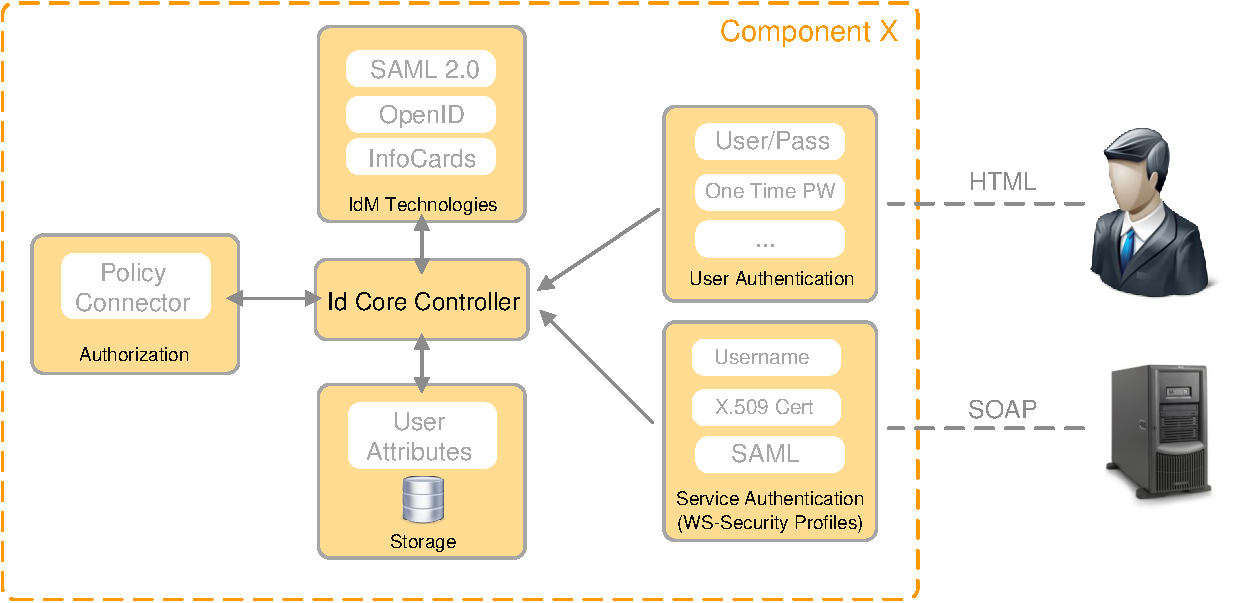
\includegraphics[width=9cm]{intro_example.pdf}\\
  %\caption{Component X}\label{fig:intro}
%\end{figure}

\section{Outline\label{sec:outline}}

This section gives a brief outline of the content of the following chapters in this
thesis.
\\
\\
\textbf{Chapter \ref{cha:relatedwork}} describes the relevant researches and the
foundation works which are used in this thesis. It also gives an introduction to the
background needed to follow the next chapter.
\\
\\
\textbf{Chapter \ref{cha:methodology}} discusses the architectural design of the model
classes we use in this thesis, how we train the models and some relevant theoretical
reasoning. The evaluation strategy and the train-test split are also thoroughly discussed.
\\
\\
\textbf{Chapter \ref{cha:evaluation}} explains how we set up the experiments and
thoroughly analyzes  the evaluation results of our models.
\\
\\
\textbf{Chapter \ref{cha:conclusion}} summarizes the thesis, describes the problems that
occurred and gives an outlook about future work.

    \chapter{Fundamentals and Related Work\label{cha:relatedwork}}

\section{Image Classification using Deep Learning}

\acrfull{dl} has a lot of advantages compared to the other \acrshort{ml} methods. First,
in many cases, it does not need a thorough and careful Feature Extraction, the techniques
such as \acrshort{cnn} help the network learn the features by itself during the training.
Second, the multiple-layer nature enable it to learn multiple levels of features from the
data. Because of that, Image Classification has been a very common domain application for
Deep Learning since the beginning, and is one of the domains where it achieved the most so
far. 

In Computer Vision, different works are usually evaluated on some standard "de facto"
labeled datasets. The accuracies on those datasets are considered as the performance
metric of a network; and those having higher scores on the datasets are considered the
better ones. ImageNet \cite{imagenet} is currently the biggest and most popular Object
Image Database available, consisting of millions of images and over 20000 object
categories. 

At the moment, there are many different approaches of Deep Learning to solve the ImageNet
Image Classification challenge. A common point of all of them is the use of the pattern
Convolutional, Max-Pooling and ReLU layers. In this section we briefly summarize the three
most popular networks which are AlexNet \cite{alexnet}, VGG \cite{vgg} and Inception
\cite{inception1, inception2, inception3}.

\begin{figure}[h]
  \centering
  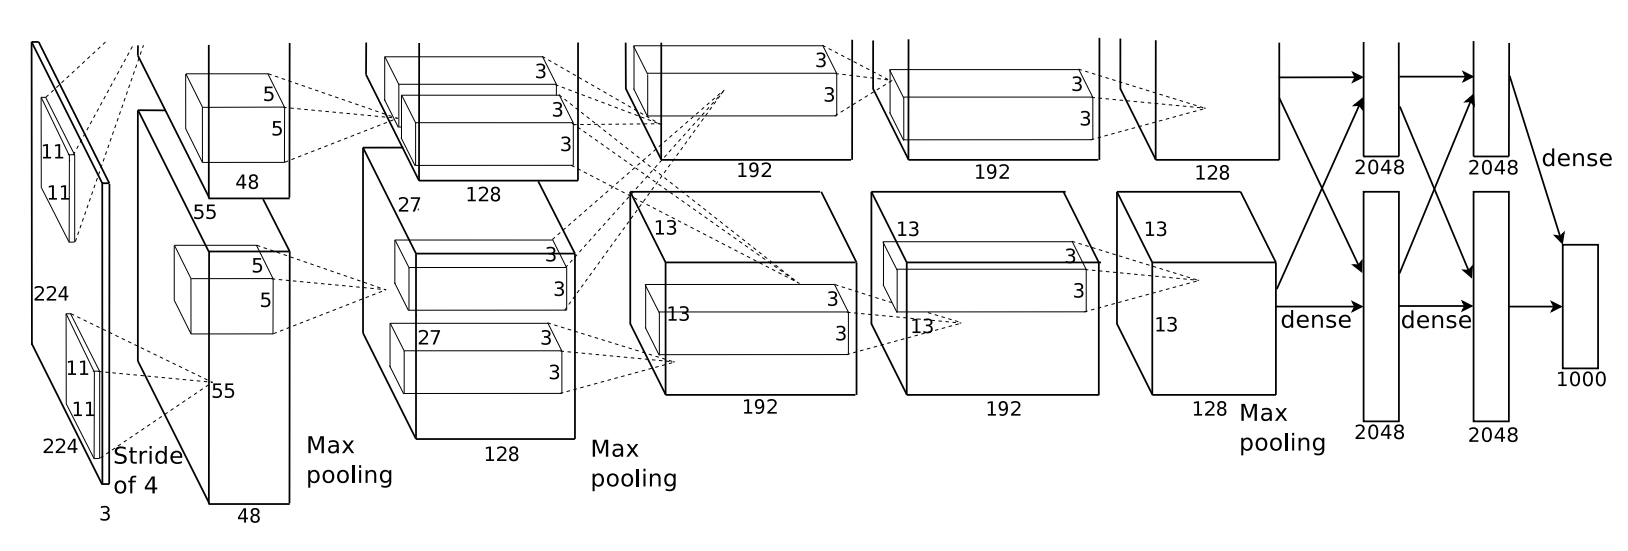
\includegraphics[width=0.9\textwidth]{alexnet_architecture}
  \caption{AlexNet Architecture \cite{alexnet}}
  \label{fig:alexnet}
\end{figure}

On ImageNet, Krizhevsky et al. \cite{alexnet} trained an 8-layer Convolutional Neural
Networks which achieved 37.5\% Top-1 error rate and 17.0\% Top-5 error rate. The network,
which is often referred as AlexNet later, was one of the first Deep Neural Networks to
improve the classification score on ImageNet significantly, and started an era that Deep
Learning leaves most of the traditional Computer Vision methods far behind. 

AlexNet consists of 8 layers as shown in Figure~\ref{fig:alexnet}. There are 5
convolutional layers and 3 fully-connected layers. The last layer is connected to a
1000-way Softmax layer because the ImageNet dataset \cite{imagenet} used to train the
network contains 1000 classes. There are different implementations on the network in
different platforms, and there are also many researches inferring the architecture, which
create small varieties of AlexNet architectures. Those differences are usually about the
size of the filters and the number of convolutional layers.

After AlexNet, there were a lot of efforts from different research groups on further
improving the classification results, resulting in many different architectures. A famous
example is VGG Net \cite{vgg}. It was introduced at the Visual Geometry Group in Oxford
and was able to achieve a Top-1 error rate of 23.7\% and Top-5 error rate of 6.8\% on
ImageNet in the best setting. The difference between VGG and AlexNet is in the filter size
and the depth of the network, which can be seen in figure \ref{fig:vgg}. Unlike AlexNet,
the authors of VGG propose a stack of three fixed filter size of $3 \times 3$ and
introduce much deeper architectures. Depending on the particular configuration, the
network can grow up to 19 layers. Despite the highly achieved ImageNet accuracies, VGG
also has big advantages which are the training time and the storage size of the network,
because of the huge depth.

\begin{figure}[h]
	\centering
	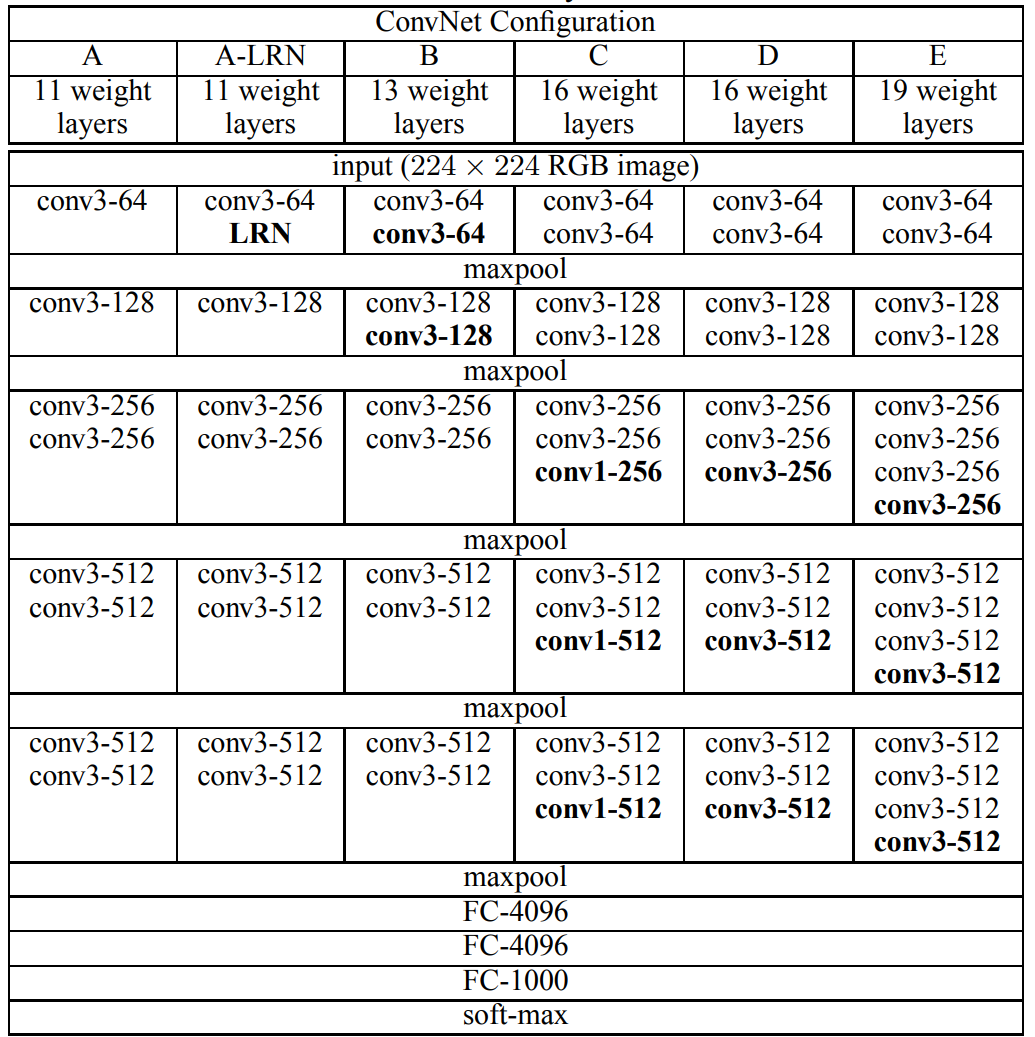
\includegraphics[width=0.8\linewidth]{vgg}
	\caption{VGG architecture and specs from the original paper \cite{vgg}}
	\label{fig:vgg}
\end{figure}

Another popular State-Of-The-Art image classification architecture is Inception
\cite{inception1}. It has quite a different design than the other two. Particularly, the
authors define a module called "Inception" and apply it multiple times in the network. As
being shown in Figure~\ref{fig:inception_module}, it uses different convolution filters at
different scales and a Pooling layer, all followed by a concatenation operation. The $1
\times 1$ convolution acts as a dimensionality reduction layer. In the overall network, a
few Inception modules are used together with other common layers such as
Convolution-MaxPool and Softmax, resulting in a network with totally 22 layers. With some
different improvements in the follow-up papers \cite{inception2, inception3}, the
Inception-v4 version could reach a Top-1 Error of 17.7\% and a Top-5 Error of 3.8\% on
ImageNet. 

\begin{figure}[h!]
	\centering
	\begin{subfigure}{0.7\textwidth}
		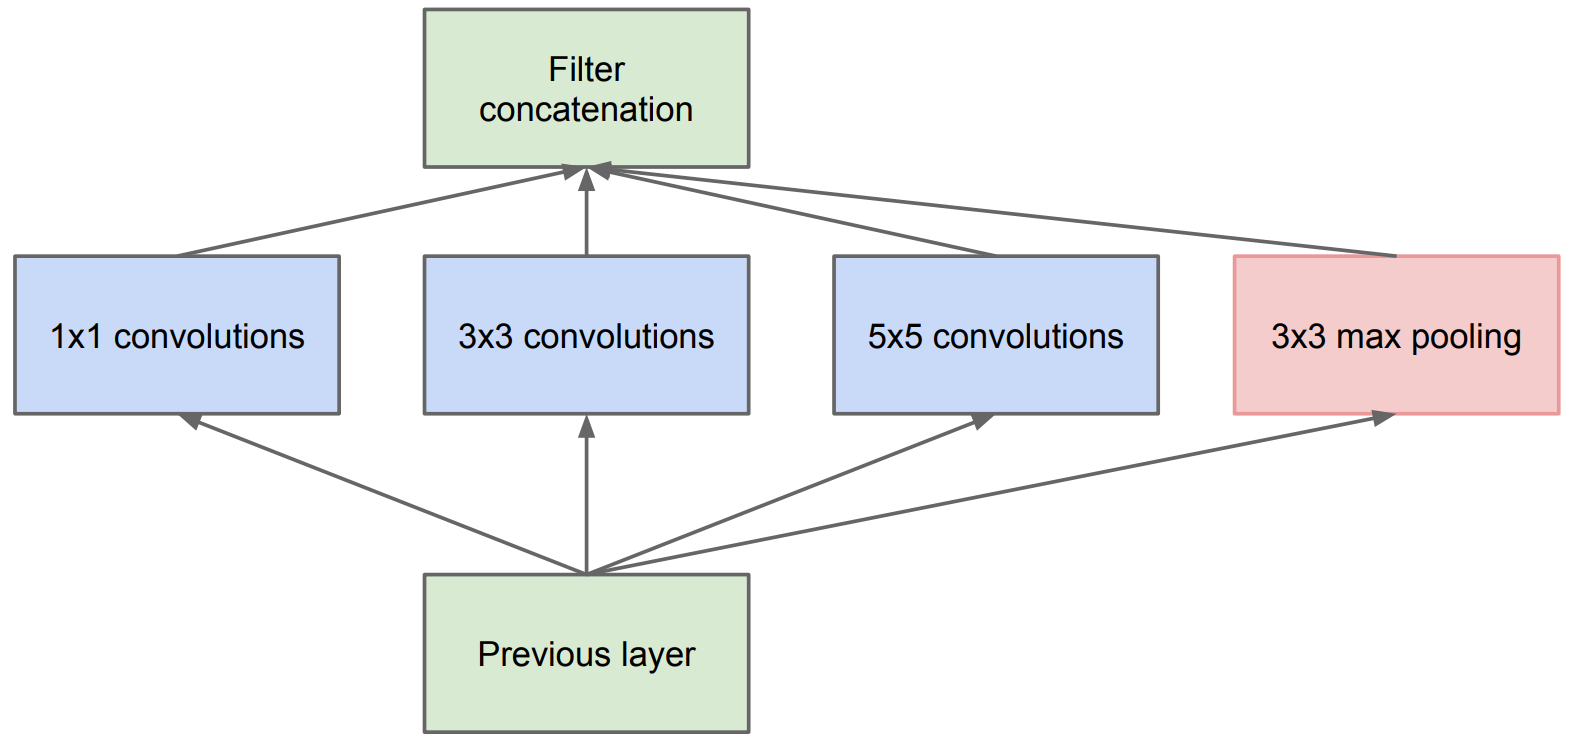
\includegraphics[width=\textwidth]{inception_module_naive}
		\caption{Inception module, naive version}
	\end{subfigure}
	\begin{subfigure}{0.7\textwidth}
		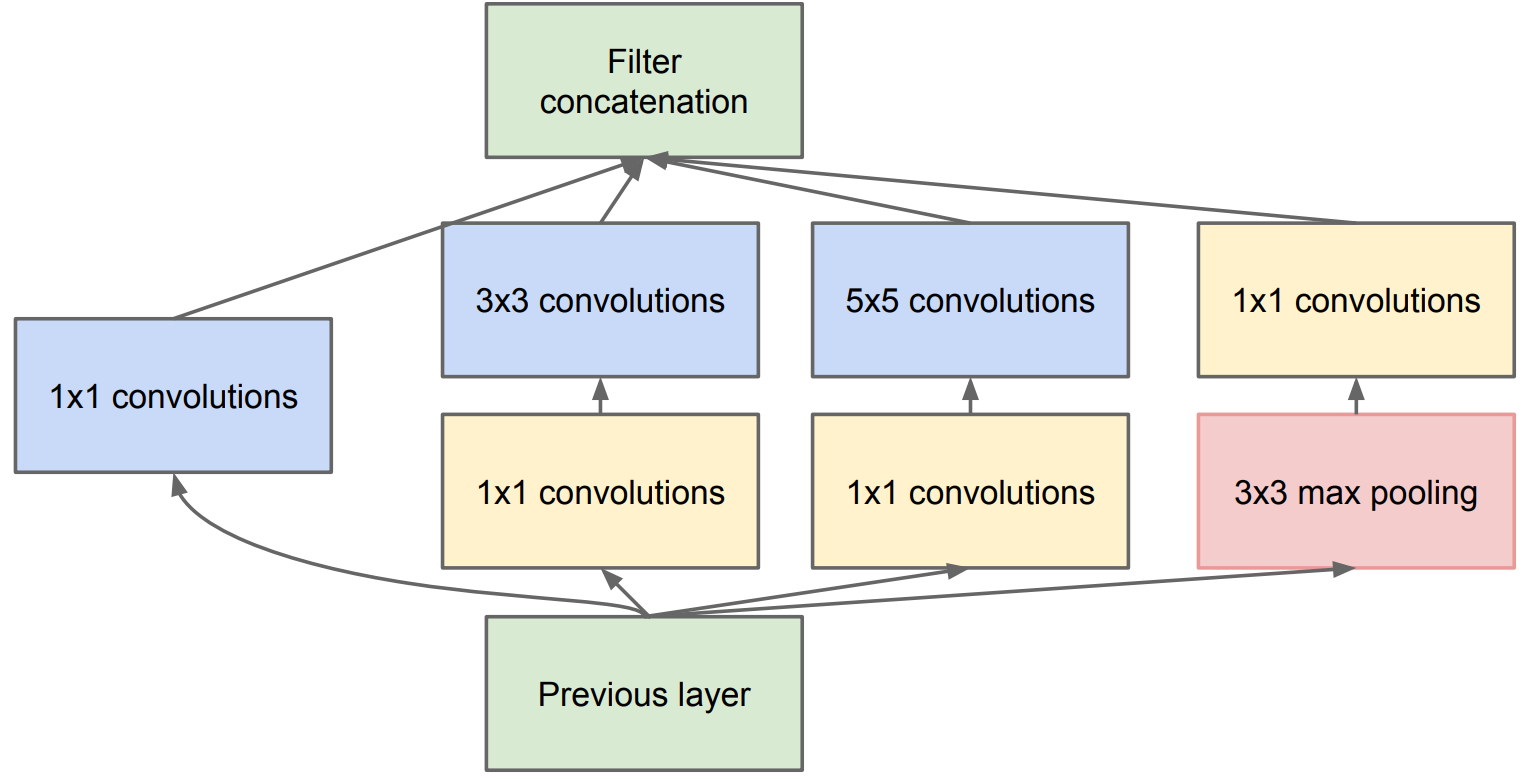
\includegraphics[width=\textwidth]{inception_module_dr}
		\caption{Inception module with dimensionality reduction}
	\end{subfigure}
	
	\caption{Inception Module from the original paper \cite{inception1}}
	\label{fig:inception_module}
\end{figure}

A common point of the three designs is that every network has a variety of different
configurations, creating different versions of the same design. People usually pick one
setting depending on the problems and the hardware power.

\subsection{Transfer Learning}

If we take a closer look at a Deep Classification Network such as AlexNet \cite{alexnet},
we can see that the last layer is often a Softmax layer, which converts the output to the
range $[0, 1]$ so that we have a prediction probability of each class. The real
classification work is done in the previous layer (fc8), where the probability that the
object image belongs to each class is calculated by a Linear Regression. In AlexNet, as we
have 1000 classes, we have 1000 neurons in fc8 corresponding to 1000 Linear Regressions.
The intuition here is that, the input of that decision layer is a good representation of
the data if the network is performing well. In principle, we can reuse the output of the
layer before fc8, which is fc7, in other \acrshort{ml} tasks.  That forms the basic idea
of Transfer Learning, which is the essential method of a number of State-Of-The-Art Object
Classifiers.

\subsection{Washington RGB-D Dataset}
\label{subsec:washington_dataset}

Beside ImageNet, the Washington RGB-D Object dataset is another one which is often used as
a "de facto" of benchmarking an Image classifier.  It is a big Image dataset introduced by
Lai ei al. \cite{washington_rgbd} at the University of Washington in Seattle. The
advantage of this dataset is that it provides depth information alongside with RGB images.
Furthermore, the RGB-D dataset is very structurally organized. Particularly:

\begin{itemize}
	\item It contains 300 common indoor objects in 51 different categories, 45 of which
		are shown in Figure~\ref{fig:washington_dataset}.
	\item Each category is then divided into different instances. For instance, in the
		"Apple" category there are 5 different apples shown in
		Figure~\ref{fig:apple_washington}.
	\item Each instance is recorded in 3 360\degree sequences by 3 different camera
		angles: 30\degree, 45\degree, and 60\degree.
	\item Each frame has:
		\begin{itemize}
			\item an RGB image of the object
			\item a Depth map
			\item a Mask indicating the	object position for extracting the object without
				background (which we do not use in this project)
			\item For every 5th frame, there is an estimated pose.
		\end{itemize}
\end{itemize}

\begin{figure}[h]
	\centering
	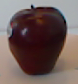
\includegraphics[height=0.10\textheight]{apple_1_1_1_crop}
	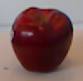
\includegraphics[height=0.10\textheight]{apple_2_1_1_crop}
	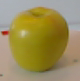
\includegraphics[height=0.10\textheight]{apple_3_1_1_crop}
	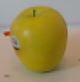
\includegraphics[height=0.10\textheight]{apple_4_1_1_crop}
	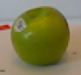
\includegraphics[height=0.10\textheight]{apple_5_1_1_crop}
	\caption{5 different instances of the "Apple" category in the Washington RGB-D object dataset}
	\label{fig:apple_washington}
\end{figure}

\begin{figure}[h]
	\centering
	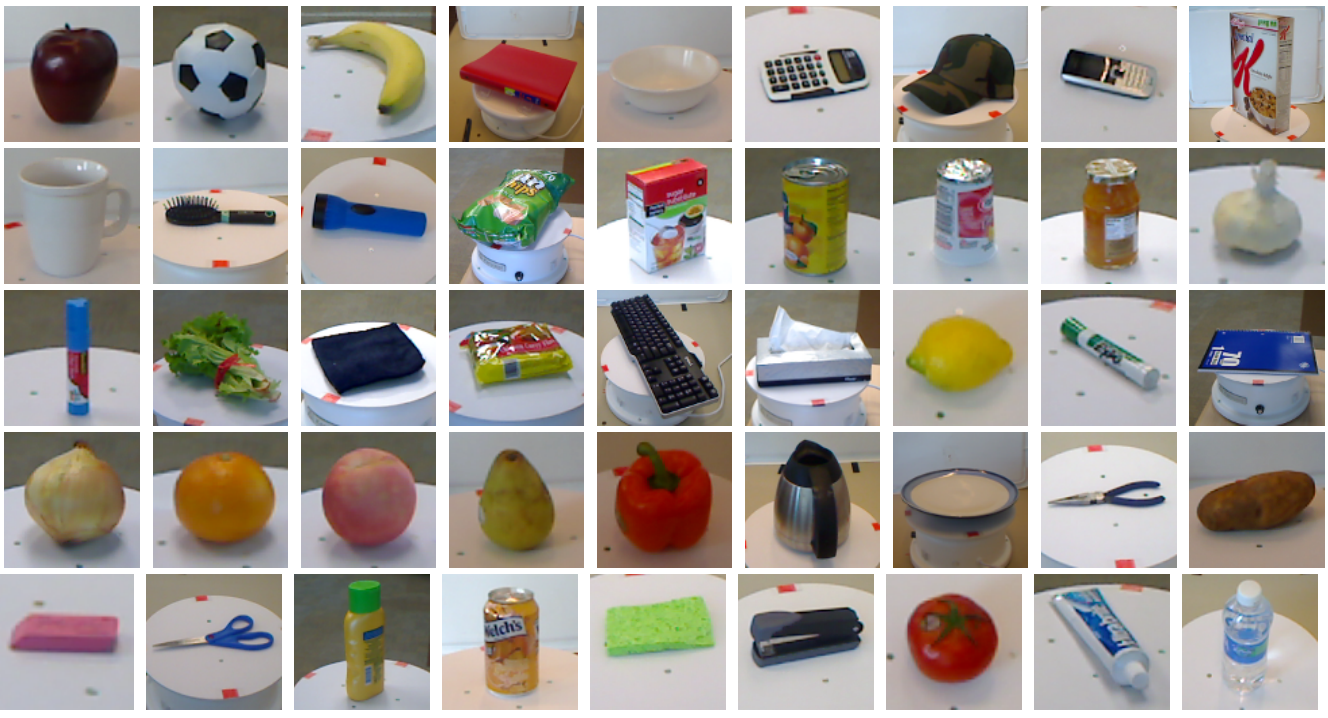
\includegraphics[width=0.8\linewidth]{washington_dataset}
	\caption{Sample RGB Images from the dataset \cite{washington_rgbd}. Each object belongs to a different
		category. Figure from the original paper. }
	\label{fig:washington_dataset}
\end{figure}

\subsection{Object Recognition on Washington RGB-D dataset}

As we have discussed in section \ref{subsec:washington_dataset}, the Washington RGB-D
Dataset has some advantages over the other ones as a "de facto" benchmarking dataset. The
biggest one is the depth maps provided alongside with the RGB frame of each item which
enables researchers to explore the potential of depth information in different
\acrshort{ml} tasks. 

The earliest work on the RGB-D Object Dataset came from the authors of the dataset
themselves \cite{lai_recognition}. They apply \acrfull{hog} to both the RGB frame and the
Depth map and propose a distance metric among different instances to do some
classifications. They achieved an accuracy of 85.4\% on the category classification task,
which was the State-Of-The-Art before the \acrshort{cnn} era.

Soon after \acrshort{cnn} was introduced, it surpassed all other traditional Computer
Vision methods. Together with the Transfer Learning techniques, the researchers quickly
got very high results on the RGB-D Object Dataset and demonstrate that depth data does
indeed reduce the classification errors \cite{eitel, alexandre}. The differences between
different approaches are usually about which pre-trained networks the authors use and how
they pre-process the image channels, especially the depth channel. In this thesis, we
build our baseline classifier based on the main components from Eitel et al.  \cite{eitel}
as it achieved high accuracies on the same dataset and the architecture is simple enough
to not take too much time to train, which is very important because we also have to train
other bigger networks (\acrshort{gan}s).

Transfer Learning is the main component of Eitel et al. \cite{eitel}. In the paper, the
authors use an implementation of AlexNet in Caffe (CaffeNet) to get the representations of
the objects in the Washington RGB-D dataset \cite{washington_rgbd}. Particularly, there
are two channels of AlexNet, one is for the RGB and the other one is for the depth-map.
The Depth-map is colorized using the jet color-map before feeding into AlexNet. The
outcome representations of both channels are then fed into a fully-connected layers, where
the final results are connected to a 51-way Softmax layer, to classify 51 different
classes in the Washington Object Dataset \cite{washington_rgbd}. Figure
\ref{fig:eitel_net} describes the network.

\begin{figure}[h]
  \centering
  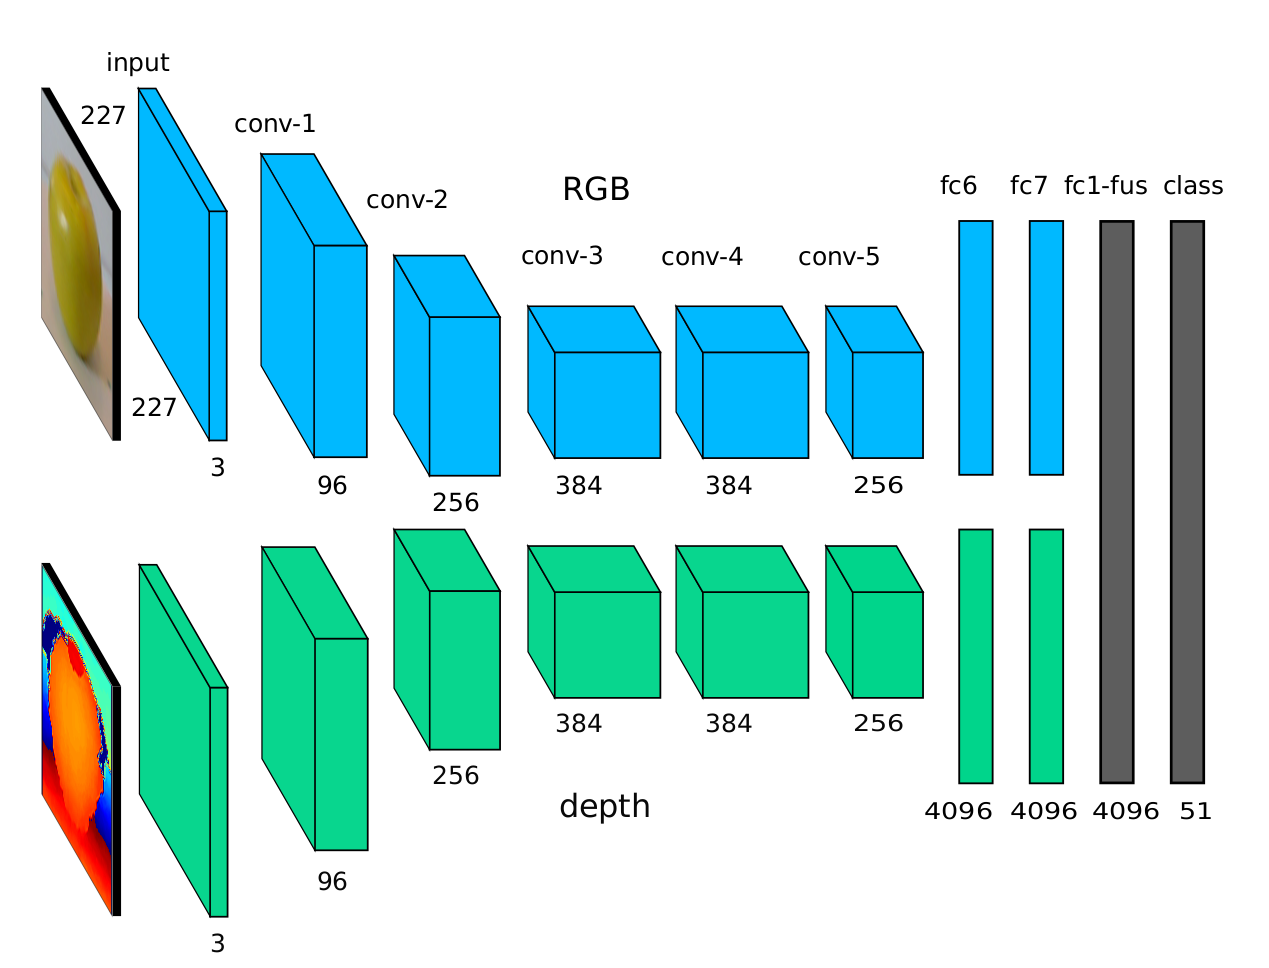
\includegraphics[width=0.8\textwidth]{eitel_net}
  \caption{Eitel et al. architecture for Object Classification. Figure from the original
	  paper \cite{eitel}}\label{fig:eitel_net}
\end{figure}

\section{\acrfull{gan}}

As being already mentioned in section \ref{subsec:intro_gan}, \acrshort{gan} consists of
two differentiable and adversarial functions: the Generator and the Discriminator, usually
in different forms of Deep Neural Networks.  

There can be different designs for the two networks depending on the domains that
\acrshort{gan}s are applied. In Computer Vision applications, it is common that the
Generator is a \acrfull{cnn} which behaves in a similar way as how an Auto Encoder
\cite{auto_encoder} works. The first half is an Encoder where an image is reduced to a
representation of 1D array, then the second half tries to decode that representation to
the original image. The difference here is that this Generator does not minimize the
direct loss between the output and the input. Instead, it tries to maximize the loss of
the Discriminator. The Discriminator, as already been explained in section
\ref{subsec:intro_gan}, is a binary classifier who tries to distinguish the original image
and the output image from the Generator. 

In the most basic setting, the Discriminator always receives a pair of inputs:

\begin{itemize}
	\item Target: The ground-truth from the dataset, also called "Real Item", label 1
	\item Output: The product of the Generator, also called "Fake Item", label 0
\end{itemize}

Let $G$ denote the generating function and $D$ denote the classification function, and
given an arbitrary image $x$, then $G(x)$ is also an image and $D(x)$ is a scalar label
where $D(x) \in {0, 1}$.

Obviously, the goal of the Discriminator is to assign label 1 for all the real images and
label 0 for all the fake images. Thus the Discriminator Loss is a Cross-Entropy between
the output of the Discriminator and the set of labels ${0, 1}$. In other words, the
Discriminator maximizes the probability of assigning the correct labels to its inputs by
maximizing the Value Function $V(D) = \log(D(x)) + \log(1 - D(G(z)))$.

At the same time, the goal of the Generator is to "create troubles" for the Discriminator.
Particularly, it tries to make the Discriminator think that its output is "real" (label
1), meaning it minimizes the second component of the Discriminator Value Function $\log(1
- D(G(z)))$.

Based on the setting above, we end up in a two-player minimax game with the 
following value function:

\begin{align*}
	\min_{G} \max_{D} V(D, G) = \mathbb{E}_{x \sim p_{data}(x)} [\log D(x)] +
	\mathbb{E}_{z \sim p_z(z)}[\log(1 - D(G(z)))]
\end{align*}

In practice, for implementation purpose, people usually set the Discriminator Loss to be
$L(D) = -V(D, G)$ so that we can use Gradient Descent to minimize it and utilize the
existing Deep Learning frameworks. The Generator is also set to maximize $\log(D(G(z)))$,
equivalent to minimizing $-\log(D(G(z)))$, instead of minimizing $\log(1 - D(G(z)))$
because the latter has problems of vanishing gradients, shown in \cite{gan}.

We can see that the Discriminator job is as simple as any other binary classifier, it
distinguishes the real data distribution $p_{data}$ from the Generator outcome
distribution $p_{g}$. In order to "fool" it, the Generator has to learn the data
distribution $p_{data}$. In every step, the optimal Discriminator is $D^{*}(x) =
\frac{p_{data}(x)}{p_{data}(x) + p_{g}(x)}$, proved in \cite{gan}. When the system reaches
an equilibrium, $p_{g}$ should converge to $p_{data}$, thus the optimal Discriminator
Outcome should be $D^*(x) = 0.5$, equivalent to a Value Function with absolute value
$|\log(0.5)+ \log(0.5)| = 1.38629436112$. This is an important property that we can use to
determine if the \acrshort{gan} training has converged or not.

As an example, if we want to learn an apple image distribution, the Generator will draw
synthesized apple images from an arbitrary input $z$, and the Discriminator will try to tell
that the output apple image is a "fake" one and an arbitrary image from the data is a "real"
one. When the two networks converge, we should have an implicit model representing an apple
image distribution.

\section{Conditional \acrshort{gan} and Pix2pix}

The original non-conditional \acrshort{gan} is sometimes referred as the "Vanilla
\acrshort{gan}". It sets up a good foundation for the field, but is sometimes unstable and
hard to train. In some applications, people are not interested in the general distribution
but rather pay attention to a directed data generation, that is, a conditional
distribution. For instance, generating a random apple may not be as interesting to somebody
as creating an image of "Pink Lady" apple. Just shortly after the introduction of
\acrshort{gan}, Mirza and Osindero \cite{cogan} proposed Conditional GANs, an improved
version of \acrshort{gan}. The idea is simple, instead of generate from an arbitrary noise
input $z$, the Generator also takes another vector $y$ as the condition. In the example of
apple image generation, we can provide a green apple image, a string "Green Apple", or a binary
label vector as $y$. The Discriminator also takes $y$ as its condition. By being trained
in that way, \acrshort{gan} now learns a conditional model $p_{g}(x|y)$ and tries to make
it as close to the conditional distribution of the data $p_{data}(x|y)$ as much as
possible. Figure \ref{fig:co_gan_model} demonstrates how conditional \acrshort{gan} works.

\begin{figure}[h]
	\centering
	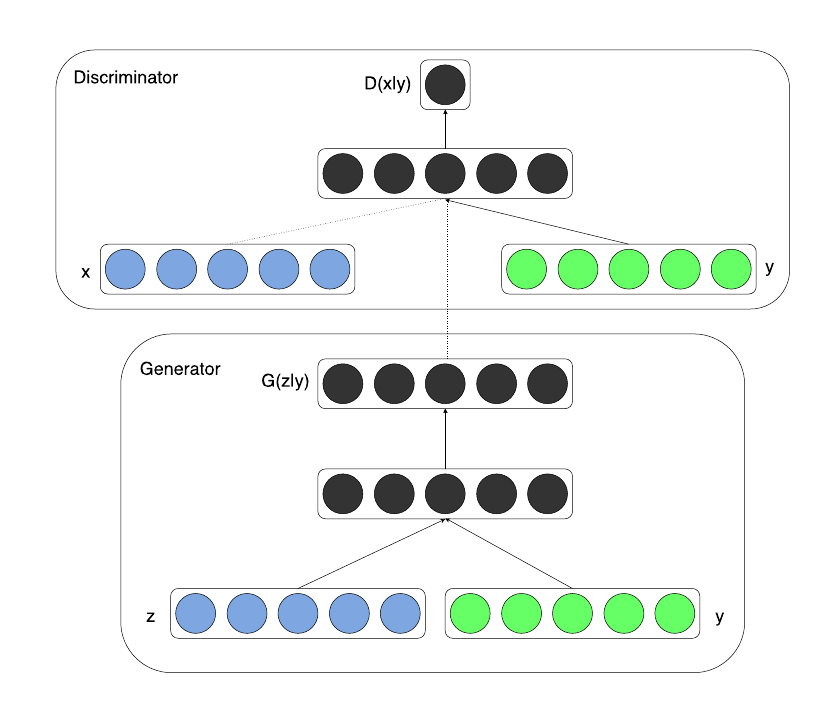
\includegraphics[width=0.5\linewidth]{img/co_gan_model}
	\caption{Conditional \acrshort{gan}s. Figure from original paper \cite{cogan}}
	\label{fig:co_gan_model}
\end{figure}

Conditional \acrshort{gan}s have many applications, one of them is image super-resolution.
The idea is to sharpen low-resolution image by converting it to a higher-resolution one.
In SRGAN \cite{sr_gan}, shown in Figure~\ref{fig:sr_gan_example}, the Generator takes a
downsampled image as the input condition and produces a higher-resolution image through a
convolutional network with some skip connections and upscaling layers; and the
Discriminator distinguishes the original input image from the output of the Generator
while being conditioned on the same downsampled image. The results were more realistic
than the other State-Of-The-Art methods, as being shown in
Figure~\ref{fig:sr_gan_example}.

\begin{figure}[h!]
	\centering
	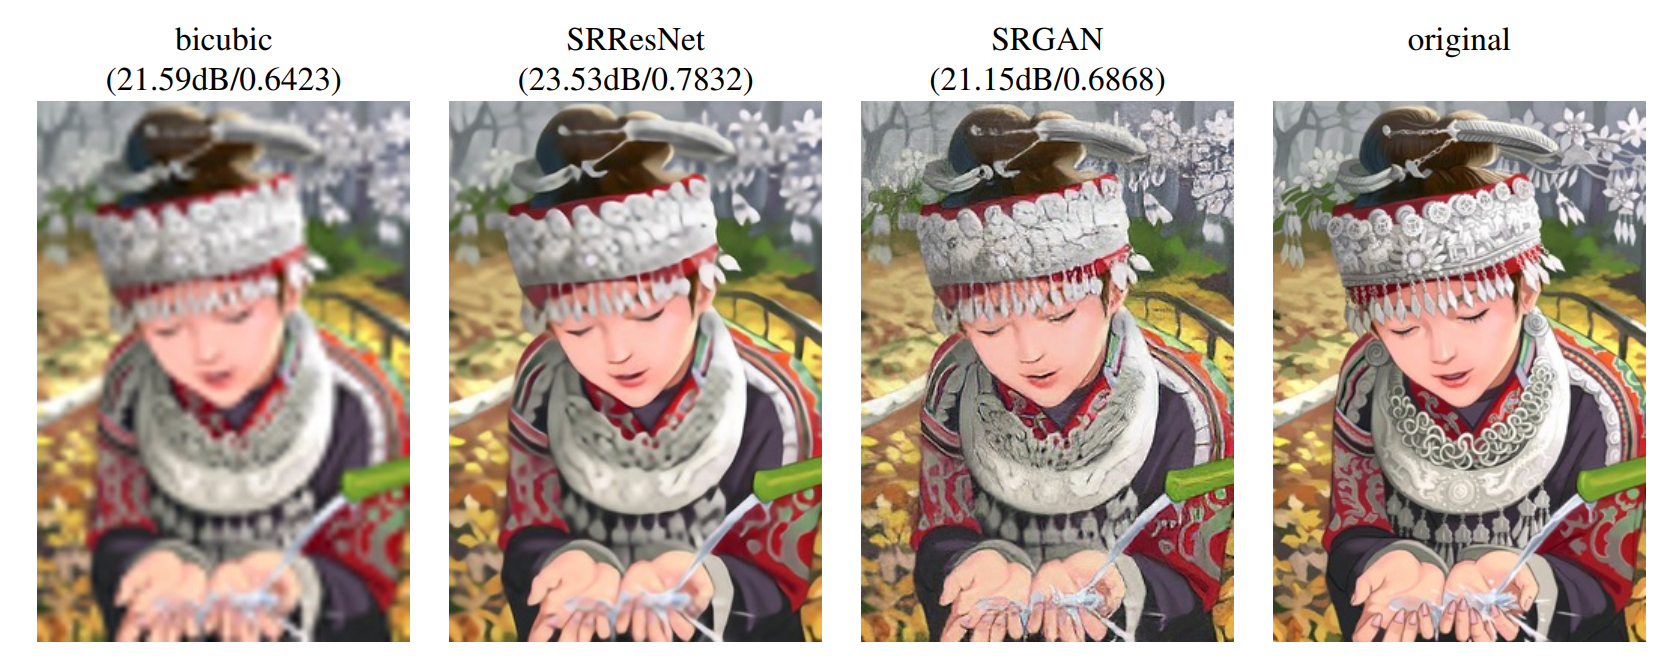
\includegraphics[width=0.8\linewidth]{sr_gan_example}
	\caption{Examples from SRGAN \cite{sr_gan}}
	\label{fig:sr_gan_example}
\end{figure}

\acrfull{pix} \cite{pix2pix} is another conditional \acrshort{gan}. It maps an image to
another image. The authors demonstrate that \acrshort{pix} is able to generate satellite
images from map views and vice versa, detailed buildings with texture from skeleton
sketches, or day to night transformation. Those impressive results come from the idea of
conditioning a \acrshort{gan} on an input image. In figure \ref{fig:pix2pix_examples}, we
can see some outputs of \acrshort{pix} from the authors.  The general workflow is
demonstrated in Figure~\ref{fig:pix2pix_workflow}.

\begin{figure}[h!]
	\centering
	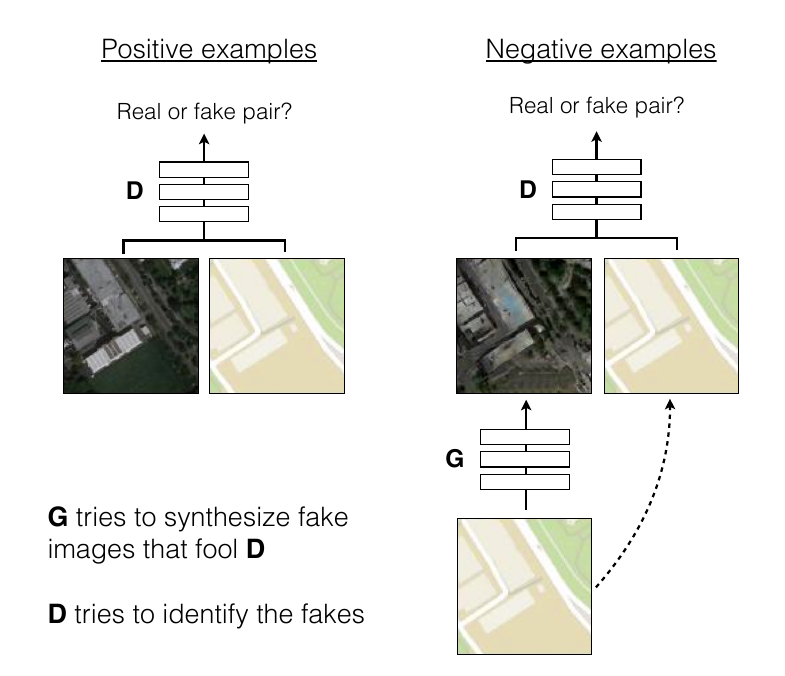
\includegraphics[width=0.5\linewidth]{img/pix2pix_workflow}
	\caption{How \acrshort{pix} works \cite{pix2pix}.}
	\label{fig:pix2pix_workflow}
\end{figure}

\begin{figure}[h!]
	\centering
	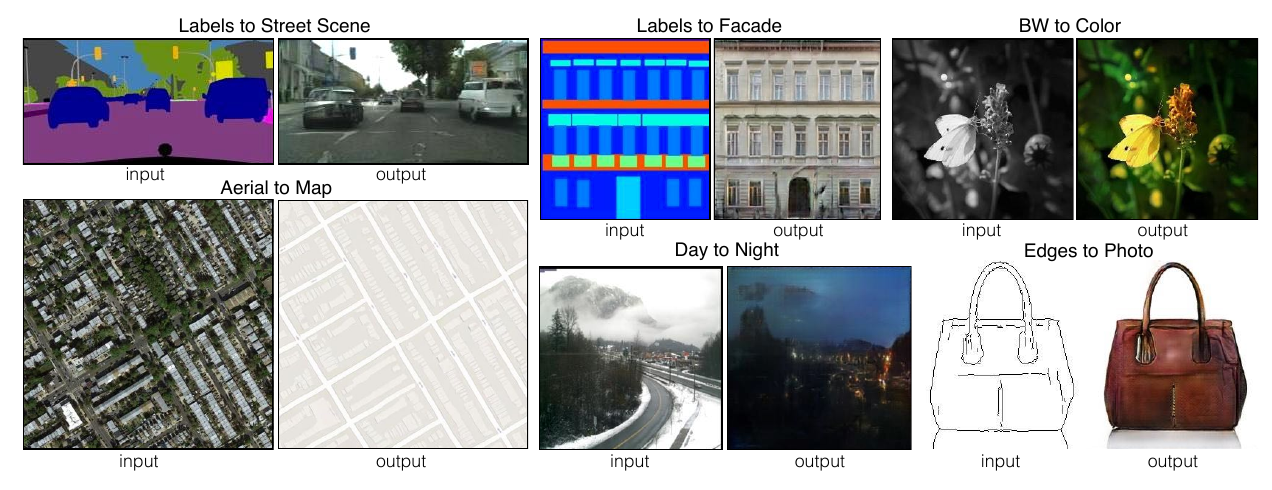
\includegraphics[width=0.8\linewidth]{img/pix2pix_examples}
	\caption{Examples of generated images from \acrshort{pix} \cite{pix2pix} }
	\label{fig:pix2pix_examples}
\end{figure}

As this is a conditional \acrshort{gan}, the loss function is also a little bit different
from the Vanilla \acrshort{gan} in the sense that all the components now are conditional
on an image $y$.  Besides, the authors also suggest using an L1 loss to boost up the
Generator training as it helps the Generator learn faster and L1 enforces less blurry
images than L2.

\begin{align*}
	\min_{G} \max_{D} V(D, G) = \mathbb{E}_{x \sim p_{data}(x)} [\log D(x, y)] +
	\mathbb{E}_{z \sim p_z(z)}[\log(1 - D(G(y, z), y))] \\ 
	+ \lambda L1(G)
\end{align*}


    \chapter{Methodology\label{cha:methodology}}
In this chapter, we describe how we design and implement the experiments with
\acrshort{gan}s to achieve the objective of the Thesis.

\section{Our \acrshort{gan}s }
The main contribution of the Thesis is to use the concept of \acrshort{gan} to
adversarially train a generative model which can produce a reasonable depth-map of a
given 2D image of a particular object. The model is expected to be able to
understand the 3D properties of images of single objects. Because of its tasks, we call
this one the "Depth-GAN".

In addition, we also train another \acrshort{gan} to learn the 3D knowledge in another
dimension, the pose estimator. This \acrshort{gan}'s job is to generate a 2D image of the
same given object in another pose. It is expected to be able to rotate, in 3D space, the
object by a particular angle while being conditioned on the object 2D image and its
corresponding depth-map. We call this one the "Pose-GAN"

\subsection{Network Architecture}

We inherit the architecture from \acrshort{pix} with only some occasional modifications in
the input and output layers because our experiments, especially the first one which
generates depth-maps from an RGB image, is very close to their settings. The detailed
settings are shown in chapter \ref{cha:model}.

The Generator is basically an U-Net \cite{u_net}, an encoder-decoder with skip
connections between every decoder layer and the corresponding encoder layer. The intuition
behind this is that, there are relevant information between the input and the output.
Especially the mirrors in the encoder part and the decoder part share the same resolution
and same level of encoding. Therefore, letting them connect directly is a good idea.
Figure~\ref{fig:u_net} visualizes the architectures of both a standard Encoder-Decoder and
U-Net.

Similarly, the Discriminator is also a Convolution-Batch-Norm-ReLu structure. It
implements an idea which the authors call "PatchGAN", where an image are divided to some
$N \times N$ patches and the network only judges the real-fake properties of each patch.
The final decision is averaged over the single-patch decisions. The rest of its job are
exactly the same as a normal binary classifier.

\begin{figure}[h]
	\centering
	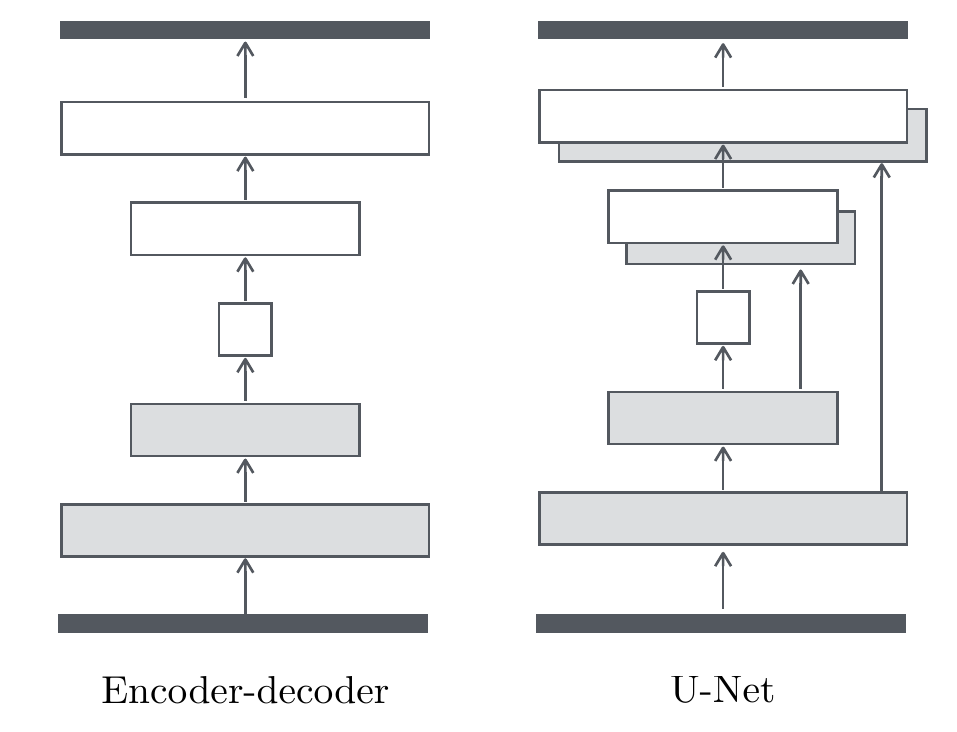
\includegraphics[width=0.6\linewidth]{u_net}
	\caption{Standard Encoder-Decoder and U-Net architectures}
	\label{fig:u_net}
\end{figure}

\subsection{Training \acrshort{gan}s}
\label{sub:training_gan}

In training \acrshort{gan}s, the Discriminator Loss is usually much more important than
the Generator Loss because it can show if the adversarial training has converged or
not. As being already explained in Chapter \ref{cha:relatedwork}, when the Discriminator
Loss is stable at 1.38629436112, we know that they two have reached an equilibrium. 

\acrshort{gan}s are notorious for being very hard to train. As it does not minimize a
simple scalar loss function, fluctuation in training is very popular and the network does
not converge eventually. This is a very hard problem and researchers are still working on
it. Fortunately, it does not always happens. Another common issue is the
Vanishing Gradient problem caused by a very quickly-converged Discriminator. In most of
the cases, the job of the Discriminator is much simpler than that of the Generator. When
its loss is too small, the gradient quickly vanishes in the Back-Propagation steps and
prevent the Generator to improve. The consequence is that the Discriminator Loss can never
reach the equilibrium of 1.38629436112.

A common method to solve this problem is to regularize the Discriminator. In this Thesis, we
occasionally apply the following tricks:

\begin{itemize}
	\item Slowing down the Discriminator by reducing its learning rate or making it wait
		for two or even more update steps of the Generator
	\item Adding instance noise to the inputs of the Discriminator. \cite{kaae}
	\item Doing One-sided Label Smoothing: replacing the label of the real image
		by a random number in a small range around 1, [0.7, 1.2] for example, instead of 1
		\cite{saliman}
\end{itemize}

While the first two methods are quite trivial as they aim to make the Discriminator job
harder to balance the work with the Generator, the third method has an interesting
explanation in Salimans et al. \cite{saliman}. The authors reuse an old concept from
several decades ago, Label Smoothing, and state that it helps reduce the sensitivity of
the network with respect to adversarial examples. The reason why we smooth only the real
samples (label 1) is that, when we apply the trick we now have the new optimal
Discriminator $D(x) = \frac{\alpha p_{data}(x) + \beta p_{model}(x)}{p_{data}(x) +
p_{model}(x)}$. When $p_{data}(x)$ is very low and $p_{model}(x)$ is very large,
$p_{model}$ has no incentive to move towards $p_{data}$. Setting $\beta = 0$, as in usual
\acrshort{gan}s, completely removes $p_{model}$ from the equation, thus prevents the
problem.

Besides, in training our Pose-GAN, we also perform another trick: removing all of the
round-shape objects, such as apple, bowl and food can. We believe that those items can
confuse the \acrshort{gan} instead of adding important values. This idea is inferred from
Elhoseiny et al. \cite{elhoseiny}, where the authors also select only 34 out of 51
categories but do not declare explicitly which categories are chosen. In our
Pose-GAN, we came up with the same number of to-be-removed categories, which are listed in
Table \ref{tab:removed_objects}.

\begin{table}[h!]
	\centering
	\caption{The round-shape objects removed from Pose-GAN training set}
	\label{tab:removed_objects}
	\begin{tabular}{@{}llllll@{}}
		\toprule
		\textbf{Category}              & \textbf{Example}      & \textbf{Category}
		& \textbf{Example}      & \textbf{Category}             & \textbf{Example}      \\
		\midrule \multicolumn{1}{|l|}{Apple}    &
		\multicolumn{1}{l|}{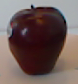
\includegraphics[height=0.08\textwidth]{apple_1_1_1_crop}} &
		\multicolumn{1}{l|}{Garlic}       &
		\multicolumn{1}{l|}{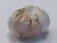
\includegraphics[height=0.08\textwidth]{garlic_1_1_1_crop}} &
		\multicolumn{1}{|l|}{Food Jar} &
		\multicolumn{1}{l|}{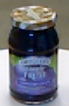
\includegraphics[height=0.08\textwidth]{food_jar_1_1_1_crop}}
		\\
		\midrule 
		\multicolumn{1}{|l|}{Peach}    &
		\multicolumn{1}{l|}{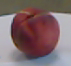
\includegraphics[height=0.08\textwidth]{peach_1_1_1_crop}} &
		\multicolumn{1}{|l|}{Tomato}   &
		\multicolumn{1}{l|}{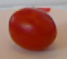
\includegraphics[height=0.08\textwidth]{tomato_1_1_1_crop}} &
		\multicolumn{1}{|l|}{Food Cup} &
		\multicolumn{1}{l|}{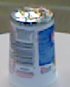
\includegraphics[height=0.08\textwidth]{food_cup_1_1_1_crop}}
		\\
		\midrule 
		\multicolumn{1}{|l|}{Food Can} &
		\multicolumn{1}{l|}{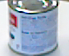
\includegraphics[height=0.08\textwidth]{food_can_1_1_1_crop}} & 
		\multicolumn{1}{l|}{Lemon}        &
		\multicolumn{1}{l|}{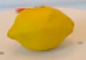
\includegraphics[height=0.08\textwidth]{lemon_1_1_1_crop}} &
		\multicolumn{1}{l|}{Glue Stick}   &
		\multicolumn{1}{l|}{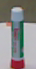
\includegraphics[height=0.08\textwidth]{glue_stick_1_1_1_crop}}
		\\
		\midrule 
		\multicolumn{1}{|l|}{Orange}   &
		\multicolumn{1}{l|}{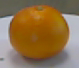
\includegraphics[height=0.08\textwidth]{orange_1_1_1_crop}} &
		\multicolumn{1}{l|}{Lime}         &
		\multicolumn{1}{l|}{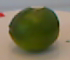
\includegraphics[height=0.08\textwidth]{lime_1_1_1_crop}} &
		\multicolumn{1}{l|}{Water Bottle} &
		\multicolumn{1}{l|}{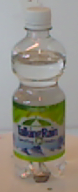
\includegraphics[height=0.08\textwidth]{water_bottle_1_1_1_crop}}
		\\
		\midrule 
		\multicolumn{1}{|l|}{Onion}    &
		\multicolumn{1}{l|}{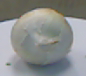
\includegraphics[height=0.08\textwidth]{onion_1_1_1_crop}} &
		\multicolumn{1}{l|}{Mushroom}     &
		\multicolumn{1}{l|}{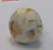
\includegraphics[height=0.08\textwidth]{mushroom_1_1_1_crop}} &
		\multicolumn{1}{l|}{Soda Can} &
		\multicolumn{1}{l|}{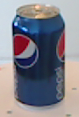
\includegraphics[height=0.08\textwidth]{soda_can_1_1_1_crop}} \\
		\midrule 
		\multicolumn{1}{|l|}{Bowl}     &
		\multicolumn{1}{l|}{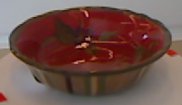
\includegraphics[height=0.08\textwidth]{bowl_1_1_1_crop}} &
		\multicolumn{1}{l|}{Plate}    &
		\multicolumn{1}{l|}{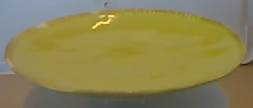
\includegraphics[height=0.08\textwidth]{plate_1_1_1_crop}} &

		&                       \\ \cmidrule(r){1-4}
	\end{tabular}
\end{table}

\subsection{Data Manipulation}

As being mentioned above, in this Thesis we focus on 2 tasks on \acrshort{gan}: learning
to generate depth information and learning to generate another pose of an object. Just to
clarify the terminologies, as we are doing image-to-image translation tasks, we call the
conditional image the "input", the to-be-generated image the "output", and the
ground-truth the "target". In that way, the Generator is supposed to make the "output" as
close to the "target" as possible, while the Discriminator still tries its best to tell
them apart.

In the first \acrshort{gan}, we line the Washington RGB-D dataset up by putting every RGB
image along with the corresponding depth-map. Here the RGB is the input, the generated
depth-map is the output, and the depth-map provided by the RGB-D dataset is the target. As
the RGB image is an 8-bit one and the depth-map is 16-bit, we have to manipulate the data
loading process to make sure that we have the correct forms. A wrong manipulation can lead
to a great loss of information.

In the additional \acrshort{gan} where we want to learn to generate a different pose of
the same object, we use both the RGB frame and the corresponding (real) depth-map as the
input condition to \acrshort{gan}, to both the Generator and Discriminator. The depth-map
is pre-processed and attached to the RGB frame as the 4th dimension, along with the three
color channels. This \acrshort{gan} will then use this information to produce a normal
3-channel RGB image of the same object, but in another pose. The Discriminator's task is
to classify this rotated image with the real image in that pose. Here the input is a
4-dimensional image, the output is an RGB, and the target is a real RGB image of that
pose.

For every frame, we choose the target pose of the 10th frame in the video sequence, which
is equivalent to a rotation of roughly 20\degree. We do that for several reasons. First,
there are subtle differences and errors among different camera scans, which makes choosing
an exact pose, such as 15\degree or 20\degree, unrealistic. Second, as we also have a
complex stratified Train-Test split which will be explained in details in section
\ref{sec:train_test_split}, we would like to make sure that the target pose of every input
frame should be in the same part of the split. A combination of an input from the training
split and a target from the test split can lead to dangerous bias in evaluation, for both
the \acrshort{gan} and the baseline classifier. Because we pick every 5th frame from every
instance to be in the test set, choosing the 10th frame as the target makes sure that the
rotated pose is in the same train-test split. Third and finally, a target rotation of
roughly 20\degree is a reasonable choice as it is big enough to observe a clear rotation
but still contains many similar details as the input, which makes the task more feasible.

For all types of \acrshort{gan}s that we are working with, the Generator produces the
Output, and the Discriminator reads both the Output and the Target and try its best to
classify the two, while both of them are conditioned on the Input. To simplify the
language, from this point we will sometimes refer both of them (i.e. the Generator and the
Discriminator) to \acrshort{gan} only. For instance, the statement "The \acrshort{gan} reads
image A and generates image B" is equivalent to "The Generator generates image B and the
Discriminator tries to distinguish image B and a target B', while both of them are
conditioned on image A"

\subsection{Handling depth missing values }

Due to technical limitations, there are corners that the sensors cannot capture the depth
information. Those values are represented as 0's in the depth-maps. If we just keep the
depth-maps as they are and feed them to the Discriminator, the \acrshort{gan} will learn
the missing value patterns and will probably somehow generate a representation of missing
values according to its understanding. This is not really what we expect; thus,
interpolating the missing values can be a good pre-processing step.

In this Thesis, we use the colorization method from a toolbox from NYU \cite{nyu_dataset},
which applies the colorization method from Levin et al. \cite{levin_colorization}. The
algorithm uses the RGB information to infer the depth values of the missing points. The
details of the optimization method can be found in the paper \cite{levin_colorization}.

\section{Baseline task}

For the baseline task, we keep most of the architecture of the 2-channel network proposed
by Eitel et al. Our implementation makes some changes on the Manipulation of the depth
missing values and the way we train the network.

In the paper, the authors propose a noise injection method to the depth-maps in the
training process. The idea is too mimic the missing values patterns (the 0 values in the
maps) so that the classifier becomes robust towards them. In other words, missing values
are considered as noise in data. In our implementation, because we also remove those
missing values from the \acrshort{gan} training process for some reasons that we have
explained in the previous section, we also do the same to the classification. Basically,
we would like the data we use to train our \acrshort{gan} and the classifier to have
identical formats.

As our approach of handling the missing values already gives better accuracies on the
original data, we do not perform fine-tuning the AlexNet channels as the authors did. A
benefit of not fine-tuning is that we can utilize the AlexNet representations for
different training rounds without re-doing back-propagation throughout the entire 9 layers
of the 2-channel network. In fact, we only train the 2 last layers for most of the
experiments.

For evaluating our Pose-GAN, we keep the same architecture, but instead of using the
colorized depth-map for the second channel, we feed the target pose of every frame. In
this way, for every item the network will receive a pair of RGB images in 2 different
pose, which we call "Stereo RGB Input". Our objective is to find out if training with 
stereo images is better than with single RGB image or not. Depth maps do not involve in
this experiment.

\section{Evaluation Method \label{sec:train_test_split}}
%\subsection{Train-Test split methodology\label{sec:train_test_split}}
As we are working on 2 Deep Learning tasks and the dataset contains many details in
different layers, a naive random Train-Test split is not the optimal approach. For this
purpose, we design a more stratified split, which is demonstrated in
Figure~\ref{fig:gan_train_test_split_depth, fig:gan_train_test_split_pose}.

For the baseline classifier, we split the data using the same strategy as in Eitel et al
\cite{eitel}, the work we refer to. In each instance, every fifth frame is sampled
and in every object, one instance is randomly and completely taken out. This gives us
about 138000 items for training and about 69000 items for testing.  We also perform the
10-cross-validation splits introduced in Lai et al \cite{washington_rgbd}. That is, each of the
lifting angle sequence is divided in to 3 sub-sequences (let us recall that each instance
in the Washington RGB-D dataset is recorded in 3 different lifting angles: 30, 45 and 60
degrees). Among those 9 sub-sequences, two are randomly added to the evaluation set. In
total, each experiment is done by using about 128000 items for training and about 78000
items for testing.

For \acrshort{gan} training, as we aim to use the \acrshort{gan} results to substitute
the real data in training the baseline classifier, we also have to design an additional
train-test split. The evaluation set generated from the previous strategy is left alone
without any further modification. Instead, we randomly split the classifier's training set
in different scales: 50-50, 25-75 and 10-90. The left portions are used for training the
\acrshort{gan} and the right portions are used to evaluate it, of which the results will
substitute the corresponding real items in the training set of the classifier. In this
way, we make sure that:

\begin{itemize}
	\item \acrshort{gan} has not seen the items it is generating samples from. In
		other words, \acrshort{gan} is in evaluation mode when being used for training the
		baseline classifier. This is important because we cannot directly use the training output
		from \acrshort{gan} to train the baseline classifier, which is bias and encourages over-fitting.
	\item We can objectively compare the classification results trained from similar
		amount of data but with different portions of real-fake components. In this way,
		we can see how \acrshort{gan} contributes to the classification accuracies in
		different scales.
\end{itemize}


\begin{figure}[h]
	\centering
	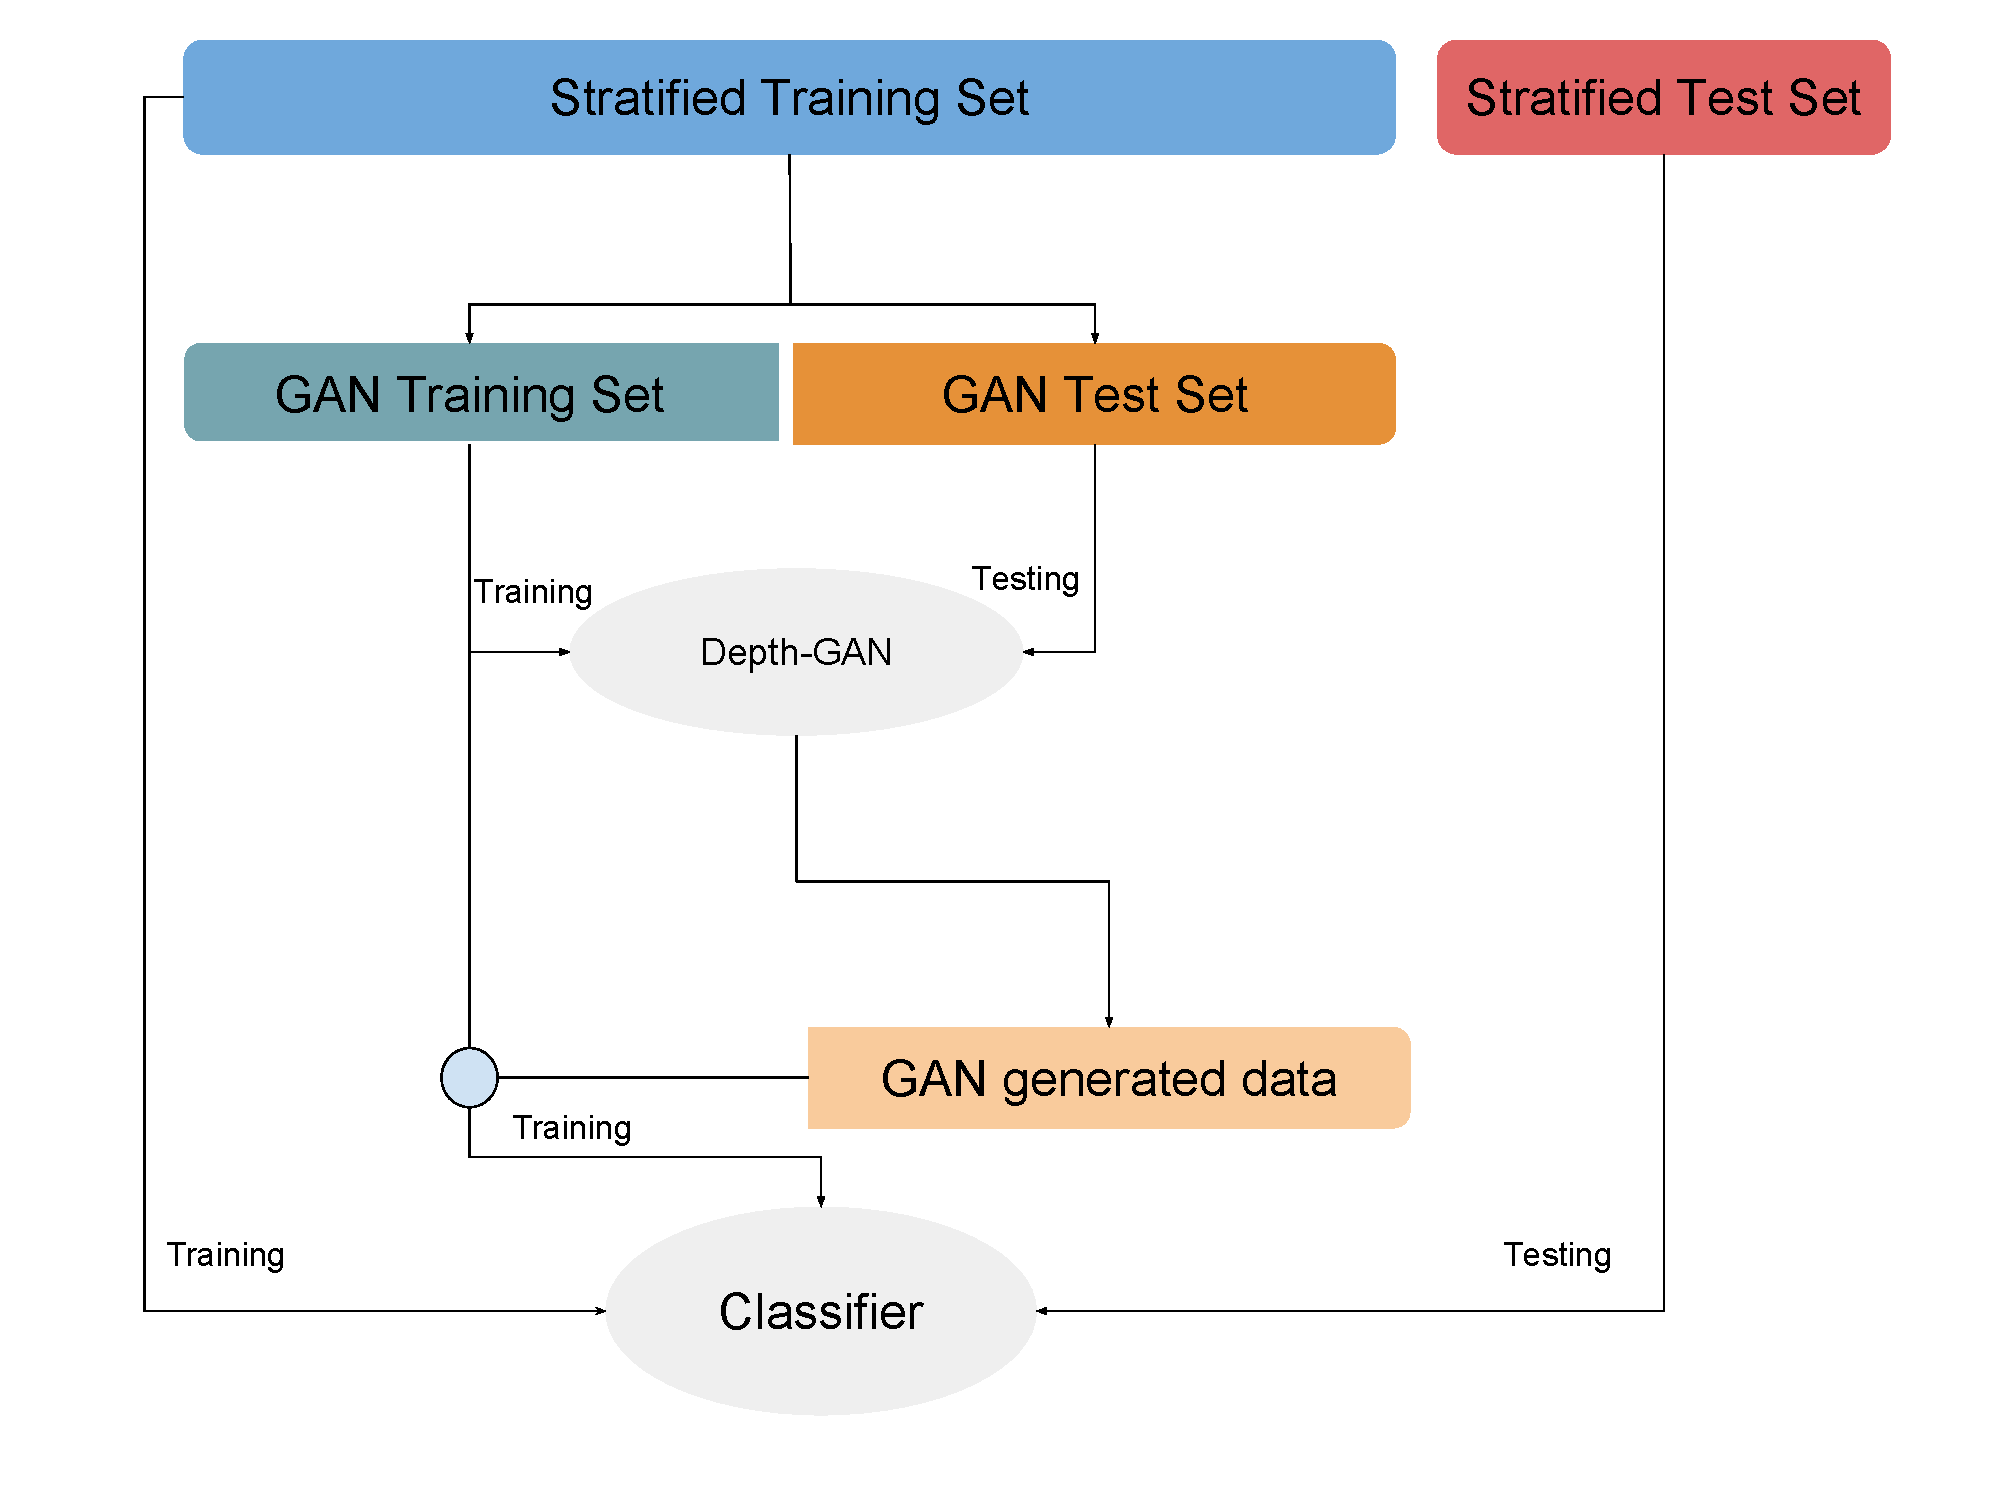
\includegraphics[width=\linewidth]{img/gan_train_test_split_depth}
	\caption{Our stratified Train-Test split for evaluating the depth-maps generation with
		\acrshort{gan}. The Stratified-Sampled Training set is split into a GAN Training
		Set and GAN Test Set with different proportions.}
	\label{fig:gan_train_test_split_depth}
\end{figure}

However, this is worth to know that this approach also has a drawback. The comparisons of
different \acrshort{gan} training setups are not entirely fair because the amounts of data
used in training the \acrshort{gan} are different. For instance, if we would like to have
90\% of \acrshort{gan} data to train the classifier, we can use only the remaining 10\% of
the data to train the \acrshort{gan} to make sure that the generated data has not been
seen by \acrshort{gan} before. However, if we keep only 50\% of \acrshort{gan} data in the
classifier's training set, we can use up to 50\% of the remaining data to train it, which
potentially results in a stronger \acrshort{gan}. 

For the Pose-GAN, the train-test split has an important difference from how we do with the
Depth-GAN. After training the \acrshort{gan}, we combine the "GAN Generated Data" with "GAN
Test Set" instead of "GAN Training Set". The reason is that our generated data now
contains all the poses supposedly in the GAN Training Set because we are doing pose
rotation. In other words, we are replacing the "GAN Training Set" by the "GAN Generated
Data". Besides, because of time limitation, we do not perform the experiments in different
scales like what we do with the Depth-GAN; only the 50-50 proportion is experimented.

\begin{figure}[h]
	\centering
	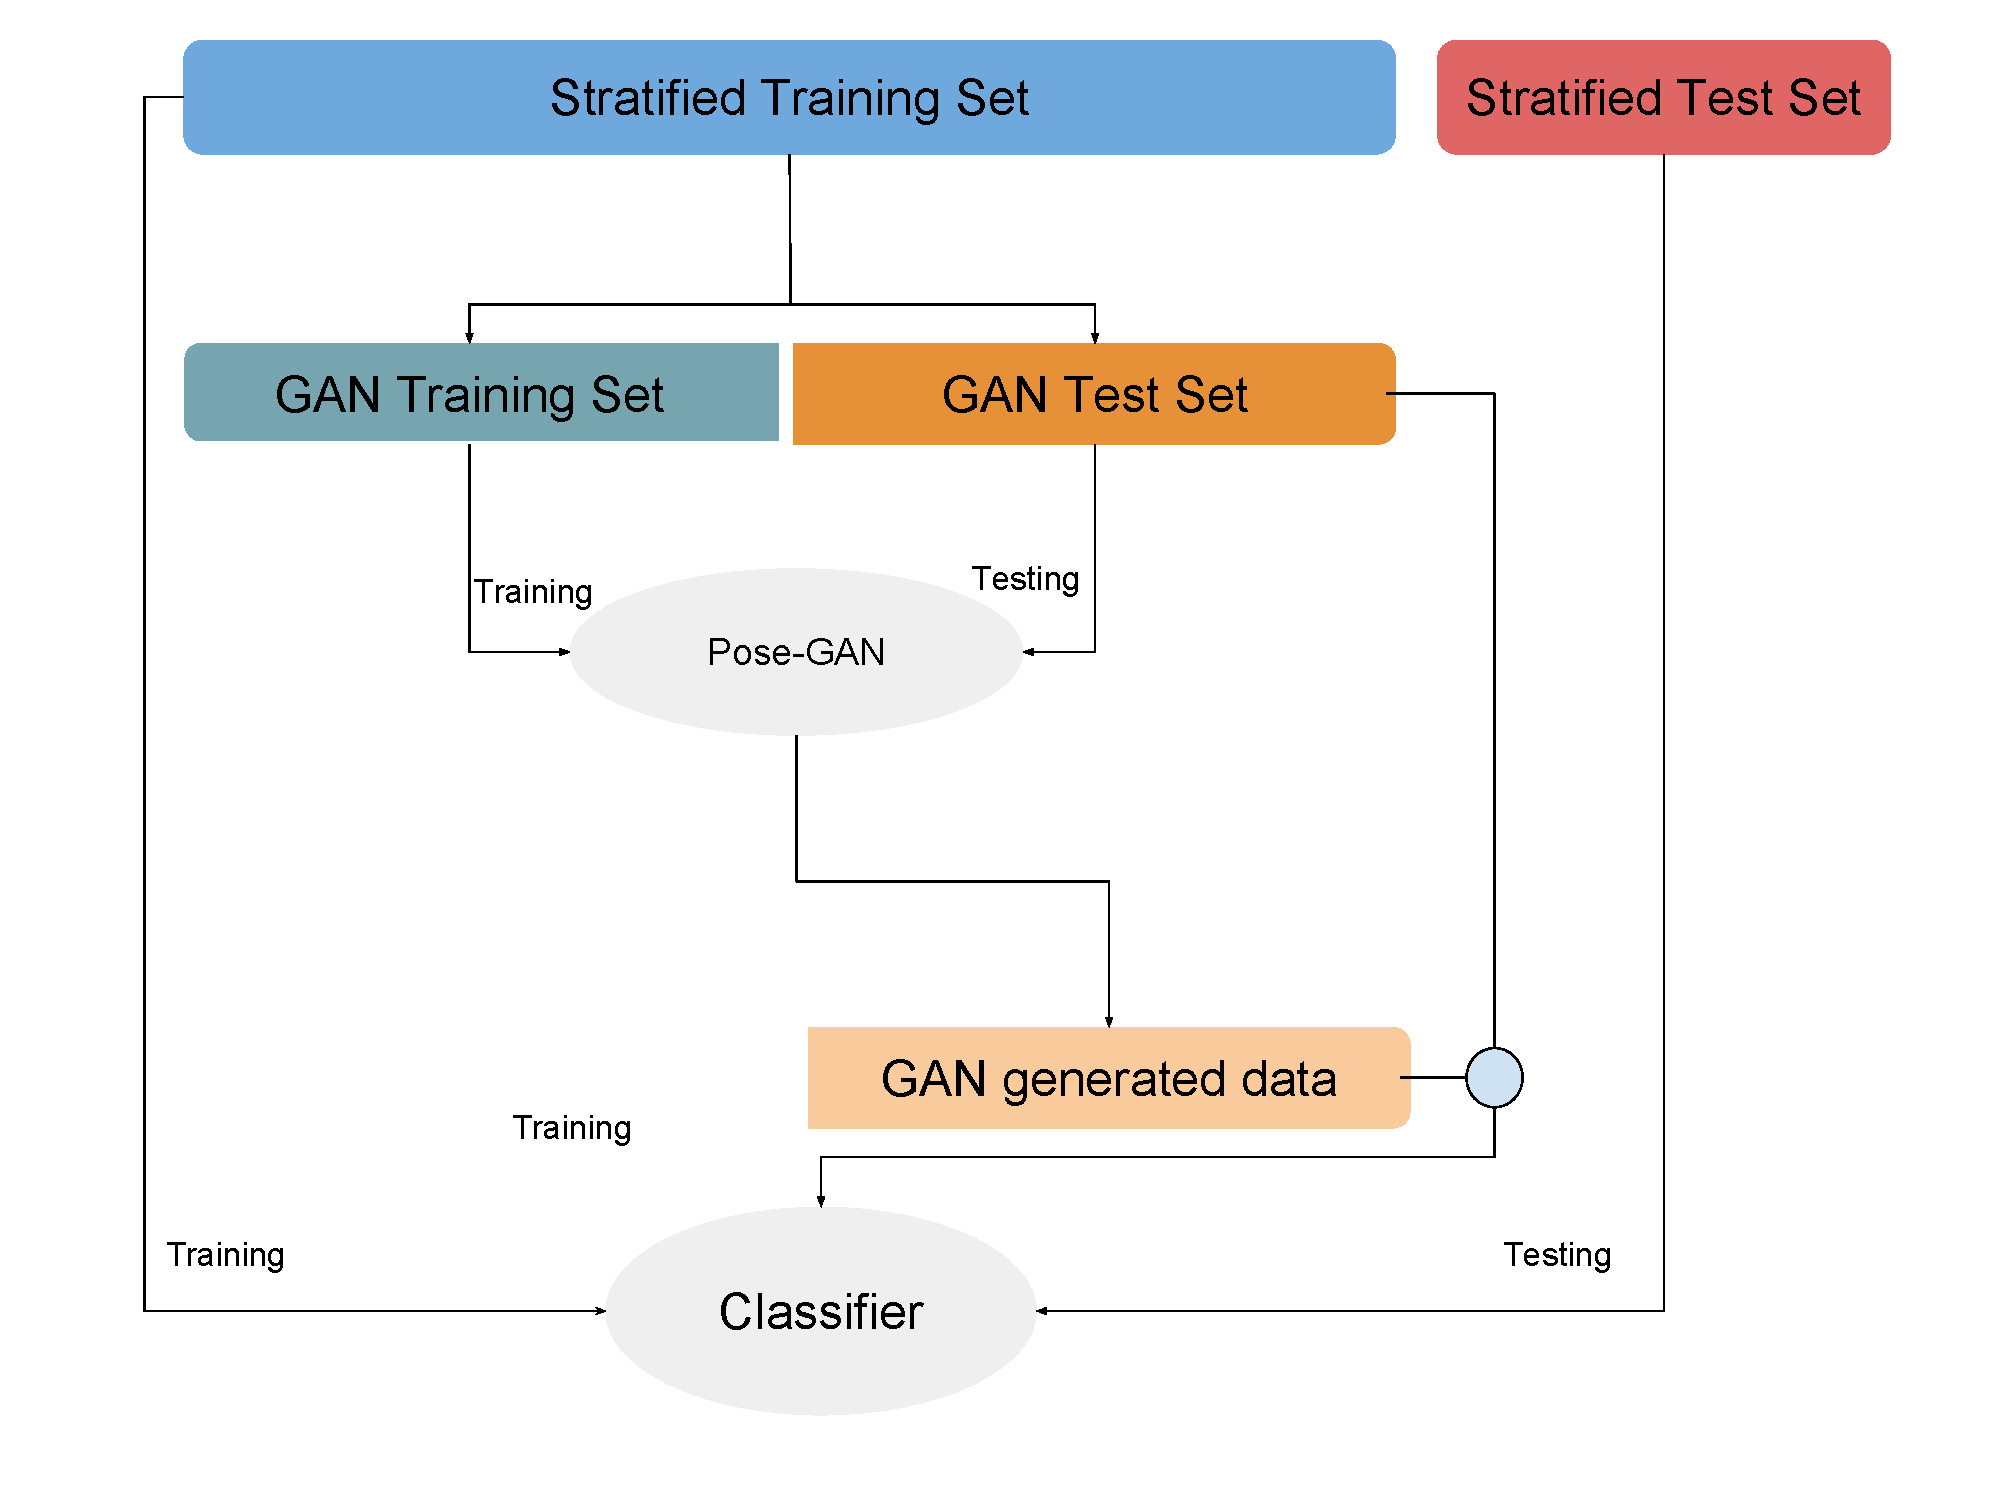
\includegraphics[width=\linewidth]{img/gan_train_test_split_pose}
	\caption{Our stratified Train-Test split for evaluating the pose generation with
		\acrshort{gan}. The Stratified-Sampled Training set is split into a GAN Training
		Set and GAN Test Set with different proportions. Note the difference here: GAN
	generated data is combined with GAN Test Set instead of GAN Training Set.}
	\label{fig:gan_train_test_split_pose}
\end{figure}

    %! TEX root = /home/duy/TUB/Thesis/latex-source/DiplomarbeitLaTex.tex

\chapter{Model}
\label{cha:model}

This short chapter is a detailed and layer-wise description of the networks we used in this Thesis.

\section{GAN Model}
\label{sec:gan_model}

Both of our \acrshort{gan}s use the architecture inherited from \acrshort{pix}
\cite{pix2pix}. Table \ref{tab:discrim} describes the layer-wise details of our
Discriminator.

\begin{table}[h]
\centering
\caption{Discriminator architecture}
\label{tab:discrim}
\begin{tabular}{|l|c|l|l|l|l|}
\hline
\multicolumn{1}{|c|}{\textbf{Layer}} & \textbf{Configuration} & \multicolumn{1}{c|}{\textbf{Filters}} & \multicolumn{1}{c|}{\textbf{Strides}} & \multicolumn{1}{c|}{\textbf{\begin{tabular}[c]{@{}c@{}}Receptive\\ Field\end{tabular}}} & \multicolumn{1}{c|}{\textbf{Comments}}                                                                                                \\ \hline
Input                                & \begin{tabular}[c]{@{}c@{}}batch\_size x \\ 256 x 256 x \\ total\_input\_channels\end{tabular} &                                       &                                       &                                                                                         & \begin{tabular}[c]{@{}l@{}}The Discriminator\\ input (GAN's output\\ or Target) is \\ concatenated\\ with the condition.\end{tabular} \\ \hline
1                                    & Convolution-ReLU                                                                                         & 64                                    & 2                                     & 4x4                                                                                     & \begin{tabular}[c]{@{}l@{}}After each layer, until \\ layer 4, the number of \\ neurons is reduced by \\ 2 times.\end{tabular}        \\ \hline
2                                    & \begin{tabular}[c]{@{}c@{}}Convolution-BatchNorm-\\ ReLU\end{tabular}                                    & 128                                   & 2                                     & 4x4                                                                                     &                                                                                                                                       \\ \hline
3                                    & \begin{tabular}[c]{@{}c@{}}Convolution-BatchNorm-\\ ReLU\end{tabular}                                    & 256                                   & 2                                     & 4x4                                                                                     &                                                                                                                                       \\ \hline
4                                    & \begin{tabular}[c]{@{}c@{}}Convolution-BatchNorm-\\ ReLU\end{tabular}                                    & 512                                   & 1                                     & 4x4                                                                                     &                                                                                                                                       \\ \hline
5                                    & Convolution-Sigmoid                                                                                      & 1                                     & 1                                     & 4x4                                                                                     &                                                                                                                                       \\ \hline
\end{tabular}
\end{table}

The Discriminator is a normal binary image classifier, so the output layer (layer 5) is a
Sigmoid producing the label (1: Real or 0: Fake) of the input image. All Leaky ReLU
functions use slope 0.2. The only variation we make is the total number of channels of the
input layers. In our Depth-GAN, we have 3 channels of the RGB frame and 1 channel of the
depth map, thus the input layer is $[batch\_size \times 256 \times 256 \times 4]$. In our
Pose-GAN, we have 4 channels of the condition (RGB and D) and 3 channels (RGB) of the
rotated frame, thus the input layer is $[batch\_size \times 256 \times 256 \times 7]$. Due
to the configuration nature of our experimental device, we usually choose $batch\_size$ to
be from 25 to 32.

\begin{table}[h]
\centering
\caption{Generator Architecture}
\label{tab:generator}
\begin{tabular}{|l|l|l|l|l|l|}
\hline
\multicolumn{1}{|c|}{\textbf{Layer}} & \multicolumn{1}{c|}{\textbf{Configuration}}                                                                            & \multicolumn{1}{c|}{\textbf{Filters}}                      & \multicolumn{1}{c|}{\textbf{Strides}} & \multicolumn{1}{c|}{\textbf{\begin{tabular}[c]{@{}c@{}}Receptive\\ Field\end{tabular}}} & \multicolumn{1}{c|}{\textbf{Comments}}                                                  \\ \hline
Input                                & \multicolumn{1}{c|}{\begin{tabular}[c]{@{}c@{}}batch\_size x \\ 256 x 256 x \\ input\_channels\end{tabular}} &                                                            &                                       &                                                                                         & \begin{tabular}[c]{@{}l@{}}The input is the \\ condition.\end{tabular}                  \\ \hline
Encoder\_1                           & \multicolumn{1}{c|}{Convolution-ReLU}                                                                                  & 64                                                         & 2                                     & 4x4                                                                                     & \begin{tabular}[c]{@{}l@{}}Output dimension: \\ 128 x 128\end{tabular}             \\ \hline
Encoder\_2                           & \multicolumn{1}{c|}{\begin{tabular}[c]{@{}c@{}}Convolution-BatchNorm-\\ ReLU\end{tabular}}                             & 128                                                        & 2                                     & 4x4                                                                                     & \begin{tabular}[c]{@{}l@{}}Output dimension: \\ 64 x 64\end{tabular}               \\ \hline
Encoder\_3                           & \multicolumn{1}{c|}{\begin{tabular}[c]{@{}c@{}}Convolution-BatchNorm-\\ ReLU\end{tabular}}                             & 256                                                        & 2                                     & 4x4                                                                                     & \begin{tabular}[c]{@{}l@{}}Output dimension: \\ 32 x 32\end{tabular}               \\ \hline
Encoder\_4                           & \multicolumn{1}{c|}{\begin{tabular}[c]{@{}c@{}}Convolution-BatchNorm-\\ ReLU\end{tabular}}                             & 512                                                        & 2                                     & 4x4                                                                                     & \begin{tabular}[c]{@{}l@{}}Output dimension: \\ 16 x 16\end{tabular}               \\ \hline
Encoder\_5                           & \multicolumn{1}{c|}{\begin{tabular}[c]{@{}c@{}}Convolution-BatchNorm-\\ ReLU\end{tabular}}                             & 512                                                        & 2                                     & 4x4                                                                                     & \begin{tabular}[c]{@{}l@{}}Output dimension: \\ 8 x 8\end{tabular}                 \\ \hline
Encoder\_6                           & \begin{tabular}[c]{@{}l@{}}Convolution-BatchNorm-\\ ReLU\end{tabular}                                                  & 512                                                        & 2                                     & 4x4                                                                                     & \begin{tabular}[c]{@{}l@{}}Output dimension: \\ 4 x 4\end{tabular}                 \\ \hline
Encoder\_7                           & \begin{tabular}[c]{@{}l@{}}Convolution-BatchNorm-\\ ReLU\end{tabular}                                                  & 512                                                        & 2                                     & 4x4                                                                                     & \begin{tabular}[c]{@{}l@{}}Output dimension: \\ 2 x 2\end{tabular}                 \\ \hline
Encoder\_8                           & \begin{tabular}[c]{@{}l@{}}Convolution-BatchNorm-\\ ReLU\end{tabular}                                                  & 512                                                        & 2                                     & 4x4                                                                                     & \begin{tabular}[c]{@{}l@{}}Output dimension: \\ 1 x 1\end{tabular}                 \\ \hline
Decoder\_8                           & \begin{tabular}[c]{@{}l@{}}ReLU-Deconvolution-\\ BatchNorm\end{tabular}                                                & 1024                                                       & 2                                     & 4x4                                                                                     & \begin{tabular}[c]{@{}l@{}}Dropout = 0.5\\ Output dimension: \\ 2 x 2\end{tabular} \\ \hline
Decoder\_7                           & \begin{tabular}[c]{@{}l@{}}ReLU-Deconvolution-\\ BatchNorm\end{tabular}                                                & 1024                                                       & 2                                     & 4x4                                                                                     & \begin{tabular}[c]{@{}l@{}}Dropout = 0.5\\ Output dimension: \\ 4 x 4\end{tabular} \\ \hline
Decoder\_6                           & \begin{tabular}[c]{@{}l@{}}ReLU-Deconvolution-\\ BatchNorm\end{tabular}                                                & 1024                                                       & 2                                     & 4x4                                                                                     & \begin{tabular}[c]{@{}l@{}}Dropout = 0.5\\ Output dimension: \\ 8 x 8\end{tabular} \\ \hline
Decoder\_5                           & \begin{tabular}[c]{@{}l@{}}ReLU-Deconvolution-\\ BatchNorm\end{tabular}                                                & 1024                                                       & 2                                     & 4x4                                                                                     & \begin{tabular}[c]{@{}l@{}}Output dimension: \\ 16 x 16\end{tabular}               \\ \hline
Decoder\_4                           & \begin{tabular}[c]{@{}l@{}}ReLU-Deconvolution-\\ BatchNorm\end{tabular}                                                & 512                                                        & 2                                     & 4x4                                                                                     & \begin{tabular}[c]{@{}l@{}}Output dimension: \\ 32 x 32\end{tabular}               \\ \hline
Decoder\_3                           & \begin{tabular}[c]{@{}l@{}}ReLU-Deconvolution-\\ BatchNorm\end{tabular}                                                & 256                                                        & 2                                     & 4x4                                                                                     & \begin{tabular}[c]{@{}l@{}}Output dimension: \\ 64 x 64\end{tabular}               \\ \hline
Decoder\_2                           & \begin{tabular}[c]{@{}l@{}}ReLU-Deconvolution-\\ BatchNorm\end{tabular}                                                & 128                                                        & 2                                     & 4x4                                                                                     & \begin{tabular}[c]{@{}l@{}}Output dimension: \\ 128 x 128\end{tabular}             \\ \hline
Decoder\_1                           & \begin{tabular}[c]{@{}l@{}}ReLU-Deconvolution-\\ Tanh\end{tabular}                                                     & \begin{tabular}[c]{@{}l@{}}Output \\ Channels\end{tabular} & 2                                     & 4x4                                                                                     & \begin{tabular}[c]{@{}l@{}}Output dimension: \\ 256 x 256\end{tabular}             \\ \hline
\end{tabular}
\end{table}

The Generator is basically a U-Net Encoder-Decoder with skip connections between the
mirrors in the Encoder part and Decoder. The detailed specs of each layer is described in
Table \ref{tab:generator}. There are 8 layers of Encoding and 8 layers of Decoding. A
Dropout of 0.5 is applied in the first 3 layers of the Decoder to create a form of
randomization in both Training and Testing. This Dropout replaces the role of the $z$
vector in Vanilla \acrshort{gan}.


\section{Object Classification Model}
\label{sec:classification_model}

As we have mentioned before, we use the model from Eitel et al. \cite{eitel}. The
architecture has been described in figure \ref{fig:eitel_net}. We extract the
representations of both RGB and Depth at the last layer of the corresponding AlexNet
tunnel, then concatenate them into a $[1 \times 8192]$ vector as the input to the fusion
network, which consists of 2 fully-connected layers. The specs of the network is described
in Table \ref{tab:fusing_network}. We train this network using the AlexNet representations
of RGB-Depth pairs from the Washington RGB-D dataset.

\begin{table}[h]
\centering
\caption{Fusing Network for Eitel et al. \cite{eitel}}
\label{tab:fusing_network}
\begin{tabular}{|l|c|l|l|}
\hline
\multicolumn{1}{|c|}{\textbf{Layer}} & \textbf{Configuration}                                                      & \multicolumn{1}{c|}{\textbf{Output}} & \multicolumn{1}{c|}{\textbf{Comments}}                                             \\ \hline
Input                                & \begin{tabular}[c]{@{}c@{}}batch\_size x \\ 8192\end{tabular}          &                                      & \begin{tabular}[c]{@{}l@{}}AlexNet representations\\ of RGB and Depth\end{tabular} \\ \hline
Fusion Layer                         & \begin{tabular}[c]{@{}c@{}}Fully Connected Layer -\\ ReLU\end{tabular}      & 1 x 4096                        & \begin{tabular}[c]{@{}l@{}}"Fusing" RGB\\ and Depth Inputs\end{tabular}            \\ \hline
Classification Layer                 & \begin{tabular}[c]{@{}c@{}}Fully Connected Layer -\\ (Softmax)\end{tabular} & 1 x 51                          & 51 classes                                                                         \\ \hline
\end{tabular}
\end{table}

    %! TEX root = /home/duy/TUB/Thesis/latex-source/DiplomarbeitLaTex.tex

\chapter{Evaluation\label{cha:evaluation}}
As we have discussed in the previous chapters, we feed the \acrshort{gan} generated data
to the two-channel Object Classification network in different proportions with respect to
the amount of original data. On one hand, we expect that \acrshort{gan}, especially the
Generator can be a good data generation engine which can help training the classification
task better. On the other hand, we hope that a well-trained classifier could be a good
tool for quantitatively evaluating \acrshort{gan} data.

In this chapter we describe how we evaluate the data generated from \acrshort{gan} using
such a baseline classifier. The basic idea is to implement the two-channel network from
Eitel et al. \cite{eitel} and compare the task's performances between using real data and
using data generated from \acrshort{gan}. Different levels of noise injection are also
used in order to evaluate how the baseline task uses depth and RGB information to make
decisions.

We train the deep classifier in the following settings:

\begin{itemize}
	\item Using the original data with both Depth and RGB information
	\item Using only a part of the original data (in different proportions) with both Depth and
		RGB information
	\item Using a part of the data (in different scales) with both Depth and RGB
		information, the remaining is substituted by \acrshort{gan} generated data
	\item Using the original data but with only RGB information in different proportions
		(10\%, 25\%, and 50\%), to determine the contribution that Depth data adds to the
		learning procedure
\end{itemize}

\section{Learning Curves}
\label{sec:learning_curves}

\acrshort{gan}s are notoriously hard to train, mainly because it does not minimize a
particular scalar function. Fluctuation and Gradient Vanishing of the Discriminator are
common problems, as being described in section \ref{sub:training_gan}. In this project,
fortunately we only face training problems with the Pose-GAN, which is acceptable because
this \acrshort{gan} actually do a much more complicated work than Depth-GAN.

The Depth-GAN's Discriminator-Loss can converge quite early to around 1.4 and becomes a
constant since then, which is a good sign because we have shown in chapter
\ref{cha:relatedwork} that the Optimal Discriminator is at the Absolute Loss of
1.38629436112. It is demonstrated in Figure~\ref{fig:depth_gan_discrim_loss}. As it
already converges, we do not need to perform any regularization here.

\begin{figure}[h!]
	\centering
	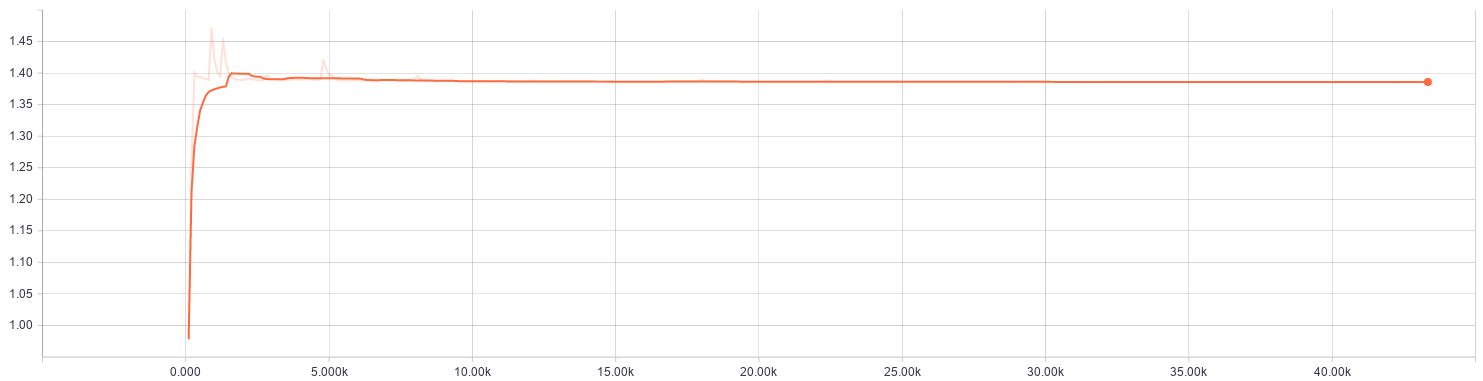
\includegraphics[width=\linewidth]{depth_gan_discrim_loss}
	\caption{The discriminator learning curve of Depth-GAN}
	\label{fig:depth_gan_discrim_loss}
\end{figure}

Things are different for the Pose-GAN, as the Generator has to do a more challenging work
so it is easy to see that the Discriminator can become very good after a short time,
causing Gradient Vanishing. It is very clear in Figure \ref{fig:pose_gan_discrim_loss}. In
the same figure, we can see that the training is much more stabilized after we perform
some regularizations. Particularly, one-sided label smoothing and instance noise injection
are very helpful. Those regularizations help the discriminator loss reaches almost 1.3,
which is much better than previously and is closer to our theoretical Optimal
Discriminator.

\begin{figure}[h!]
	\centering
	
	\begin{subfigure}{\textwidth}
		\begin{center}
			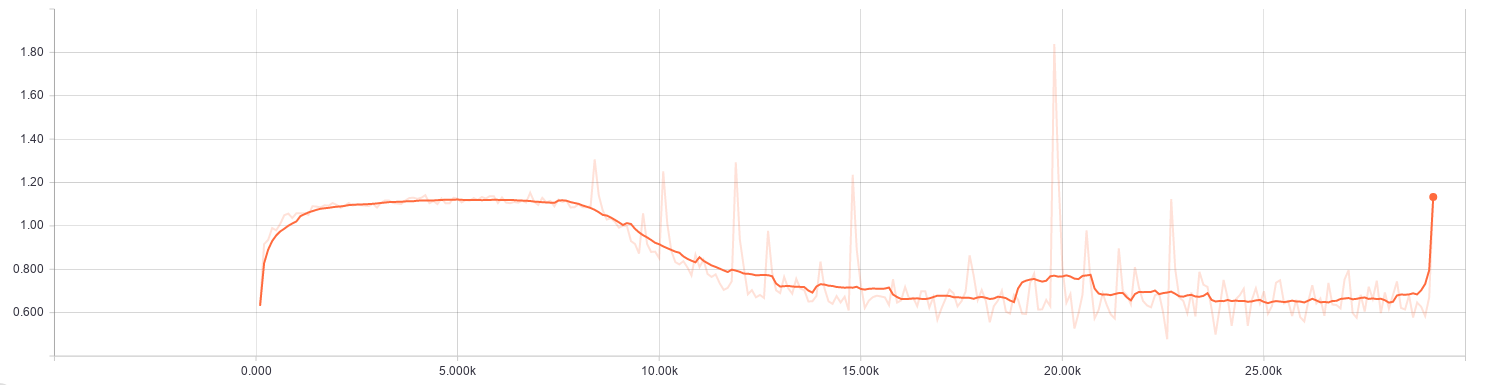
\includegraphics[width=\linewidth]{pose_gan_discrim_loss_no_regularization}
		\end{center}
		\caption{The discriminator learning curve of Pose-GAN, without any regularization}
	\end{subfigure}

	\begin{subfigure}{\textwidth}
		\begin{center}
			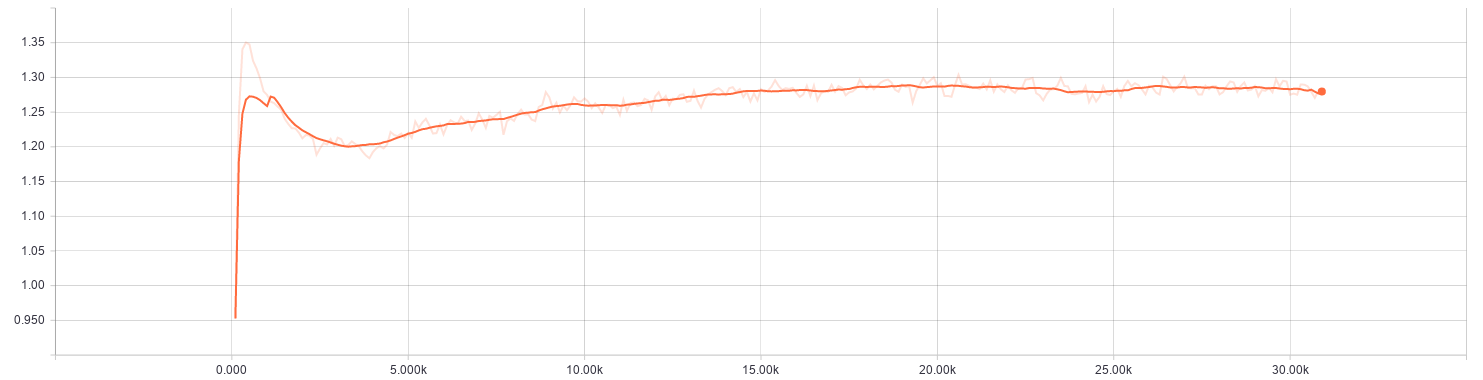
\includegraphics[width=\linewidth]{pose_gan_discrim_loss_regularized}
		\end{center}
		\caption{The discriminator learning curve of Pose-GAN, with slower learning rate,
		input instance noise, and label smoothing}
	\end{subfigure}
	\caption{Pose-GAN's Discriminator Learning Curves}
	\label{fig:pose_gan_discrim_loss}
\end{figure}

\section{Results}
\label{sec:results}

Before going to quantitative measurements, it is worthy to take a look as what our
\acrshort{gan}s produce.

\subsection{Depth-GAN}
\label{sub:depth_gan}

In Figure~\ref{fig:gan_depth}, 5 random samples from 5 random categories in the dataset
are the outputs from our Depth-GAN in Evaluation Mode, which means the corresponding
\acrshort{gan} did not see those samples in the training process.  We show the results
from all the three versions that we trained: Using 50\%, 25\% and 10\% of training data.
The depth maps are all colorized using the jet color-map for visualization purpose. It is
easy to see that the \acrshort{gan} produces very reasonable depth maps with a smooth
range of values. It is also important to see that when we reduce the amount of training
data from 50\% to 25\% and 10\%, the quality of the synthesized depth maps also noticeably
reduces. The latter Depth-GANs produce images with more noise; but they still have decent
details. This is understandable as we have explained in section
\ref{sec:train_test_split}.

Taking a look at those maps, we can see that the \acrshort{gan} does learn some trivial
knowledge. For instance, the bottom pixels tend to be closer to the sensor than the pixels
at the top of the image; and when there is a sharp edge or a sudden change of color
patterns, there is usually an object placed on top of another. We can clearly see the
second property in the sample of the fruits and the keyboard in Figure~\ref{fig:gan_depth}.

In these sample outputs from our Depth-GAN, we also see another popular advantage of
\acrshort{gan} which is already discussed in some other works \cite{gan, cogan, pix2pix}.
That is, the edges in the synthesized images are very sharp. If we instead minimized a
squared loss function for example, we could expect a much more blurry outcome. It is also
one of the reasons that using common scalar error functions such as \acrshort{mse} is not
a good way to evaluate \acrshort{gan}s' results.

\clearpage

\begin{figure}[h!]
	\centering
	\begin{subfigure}{0.8\textwidth}
		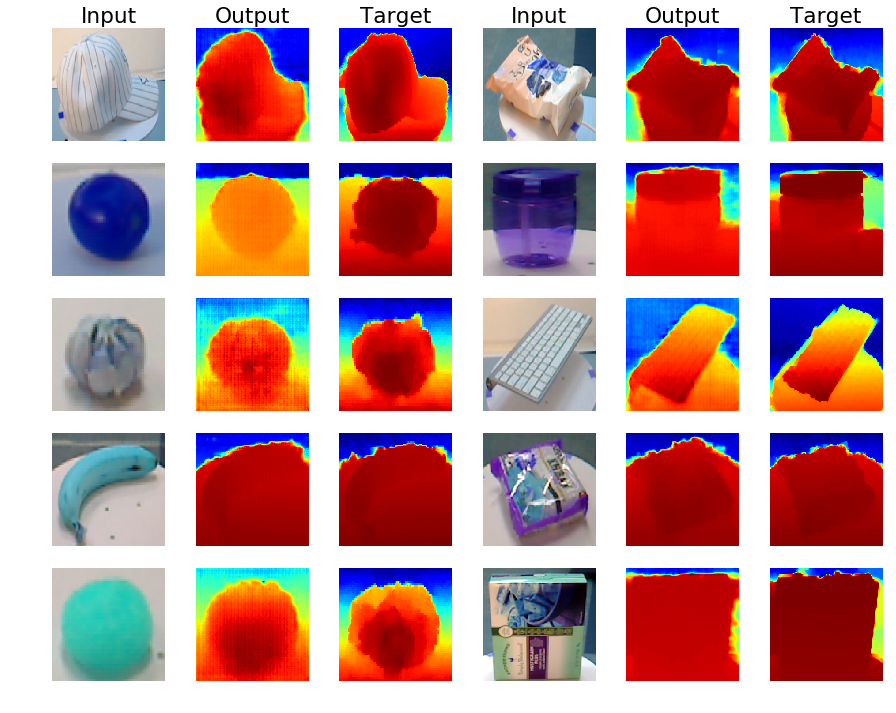
\includegraphics[width=\textwidth]{gan_depth_samples_50}
		\caption{Depth-GAN trained with 50\% data} 
	\end{subfigure}
	\begin{subfigure}{0.49\textwidth}
		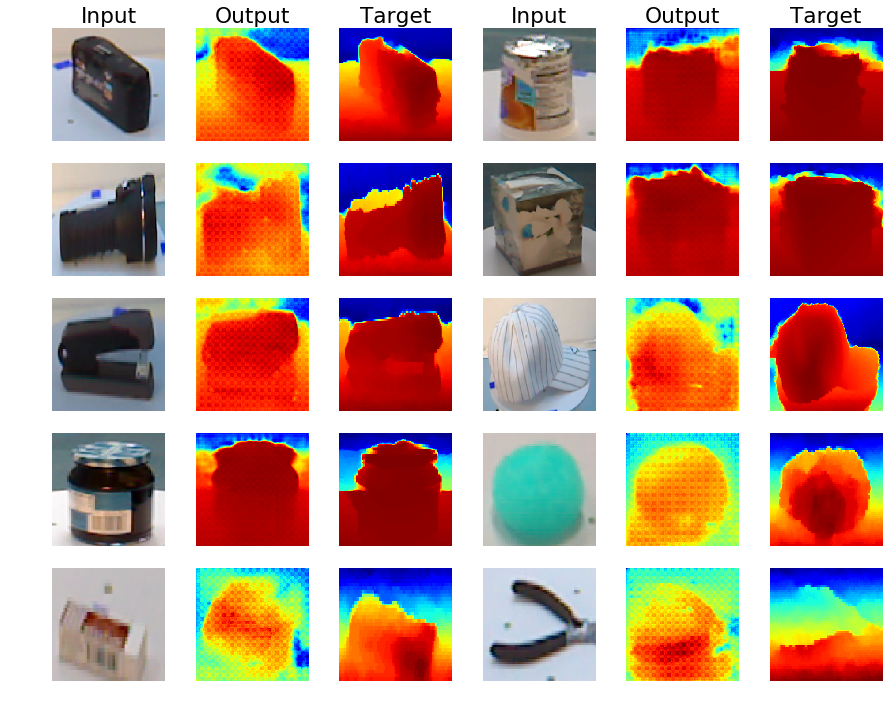
\includegraphics[width=\textwidth]{gan_depth_samples_25}
		\caption{Depth-GAN trained with 25\% data} 
	\end{subfigure}
	\begin{subfigure}{0.49\textwidth}
		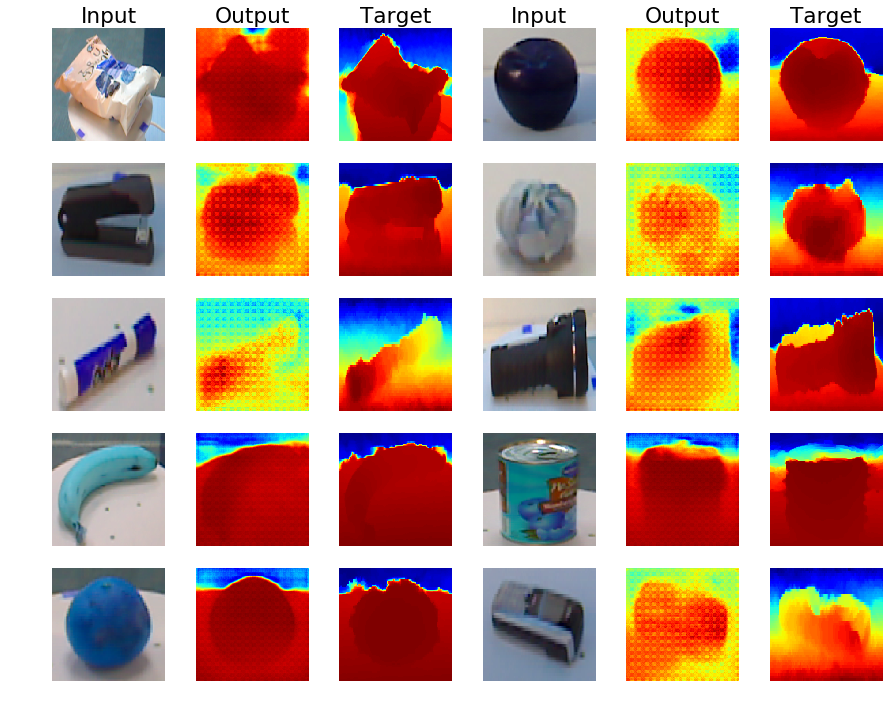
\includegraphics[width=\textwidth]{gan_depth_samples_10}
		\caption{Depth-GAN trained with 10\% data} 
	\end{subfigure}
	
	%\centering
	%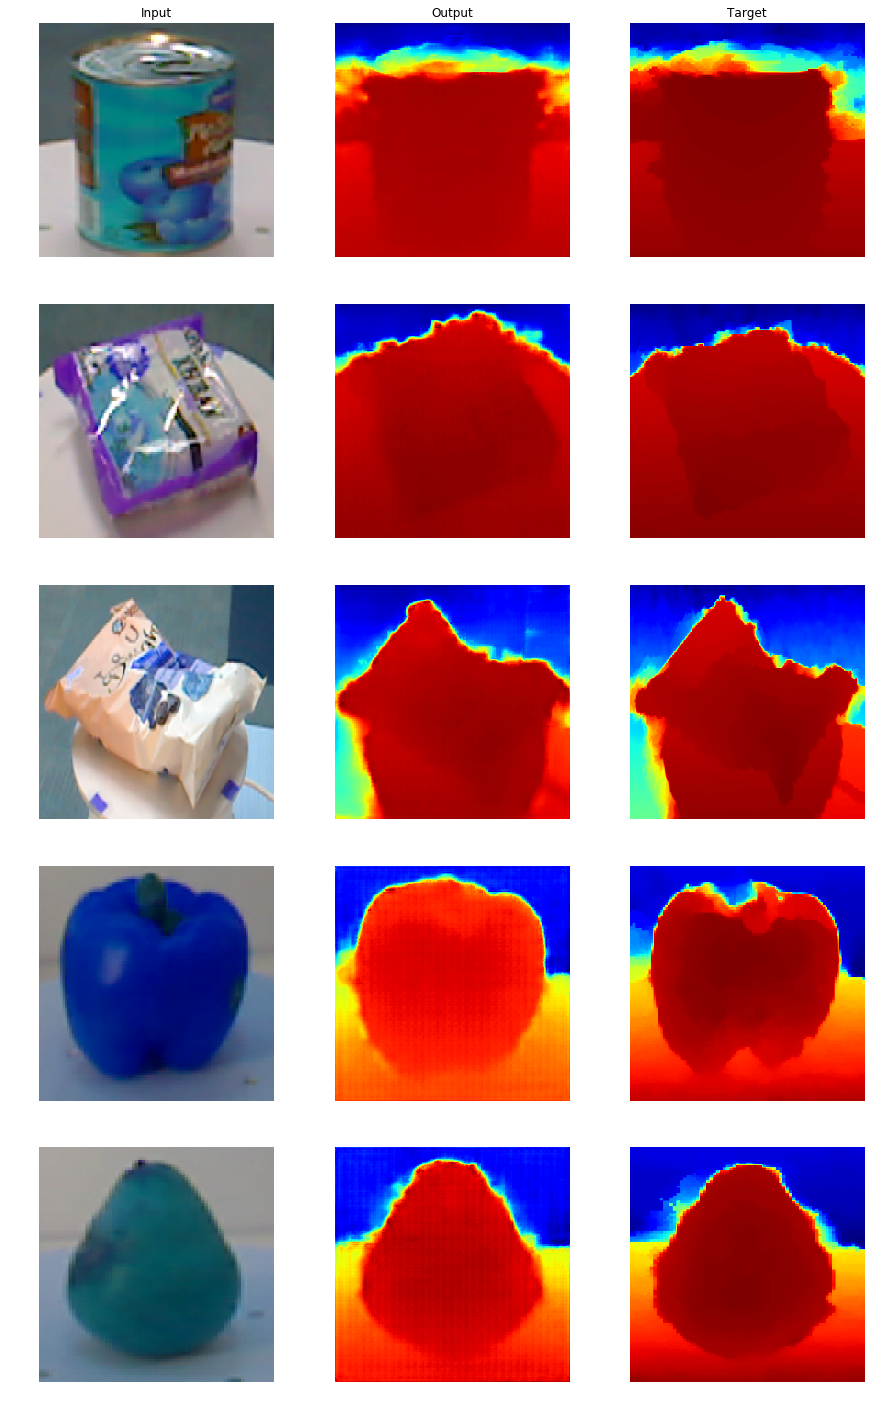
\includegraphics[width=0.72\linewidth]{gan_depth_samples}
	\caption{Some generated samples from Depth-GAN. The Output and the Target are colorized using the jet color-map.}
	\label{fig:gan_depth}
\end{figure}

\subsection{Pose-GAN}
\label{sub:pose_gan}

Similarly to the section above, Figure~\ref{fig:gan_pose_samples} shows some examples
generated from our Pose-GAN. Visually, the Outputs do not look too bad, some of them, such
as the cell phone, the flashlight and the boxes, are clearly rotated. However, the details
are clearly not optimal, and it works better with round-shape objects because they look
the same in different points of view. The overall feeling is that, the synthesized objects
are acceptable in terms of human eyes, but there is a certain level of noise in those
images, which means the Generator is still somehow confused with the given
condition/input.

\begin{figure}[h!]
	\centering
	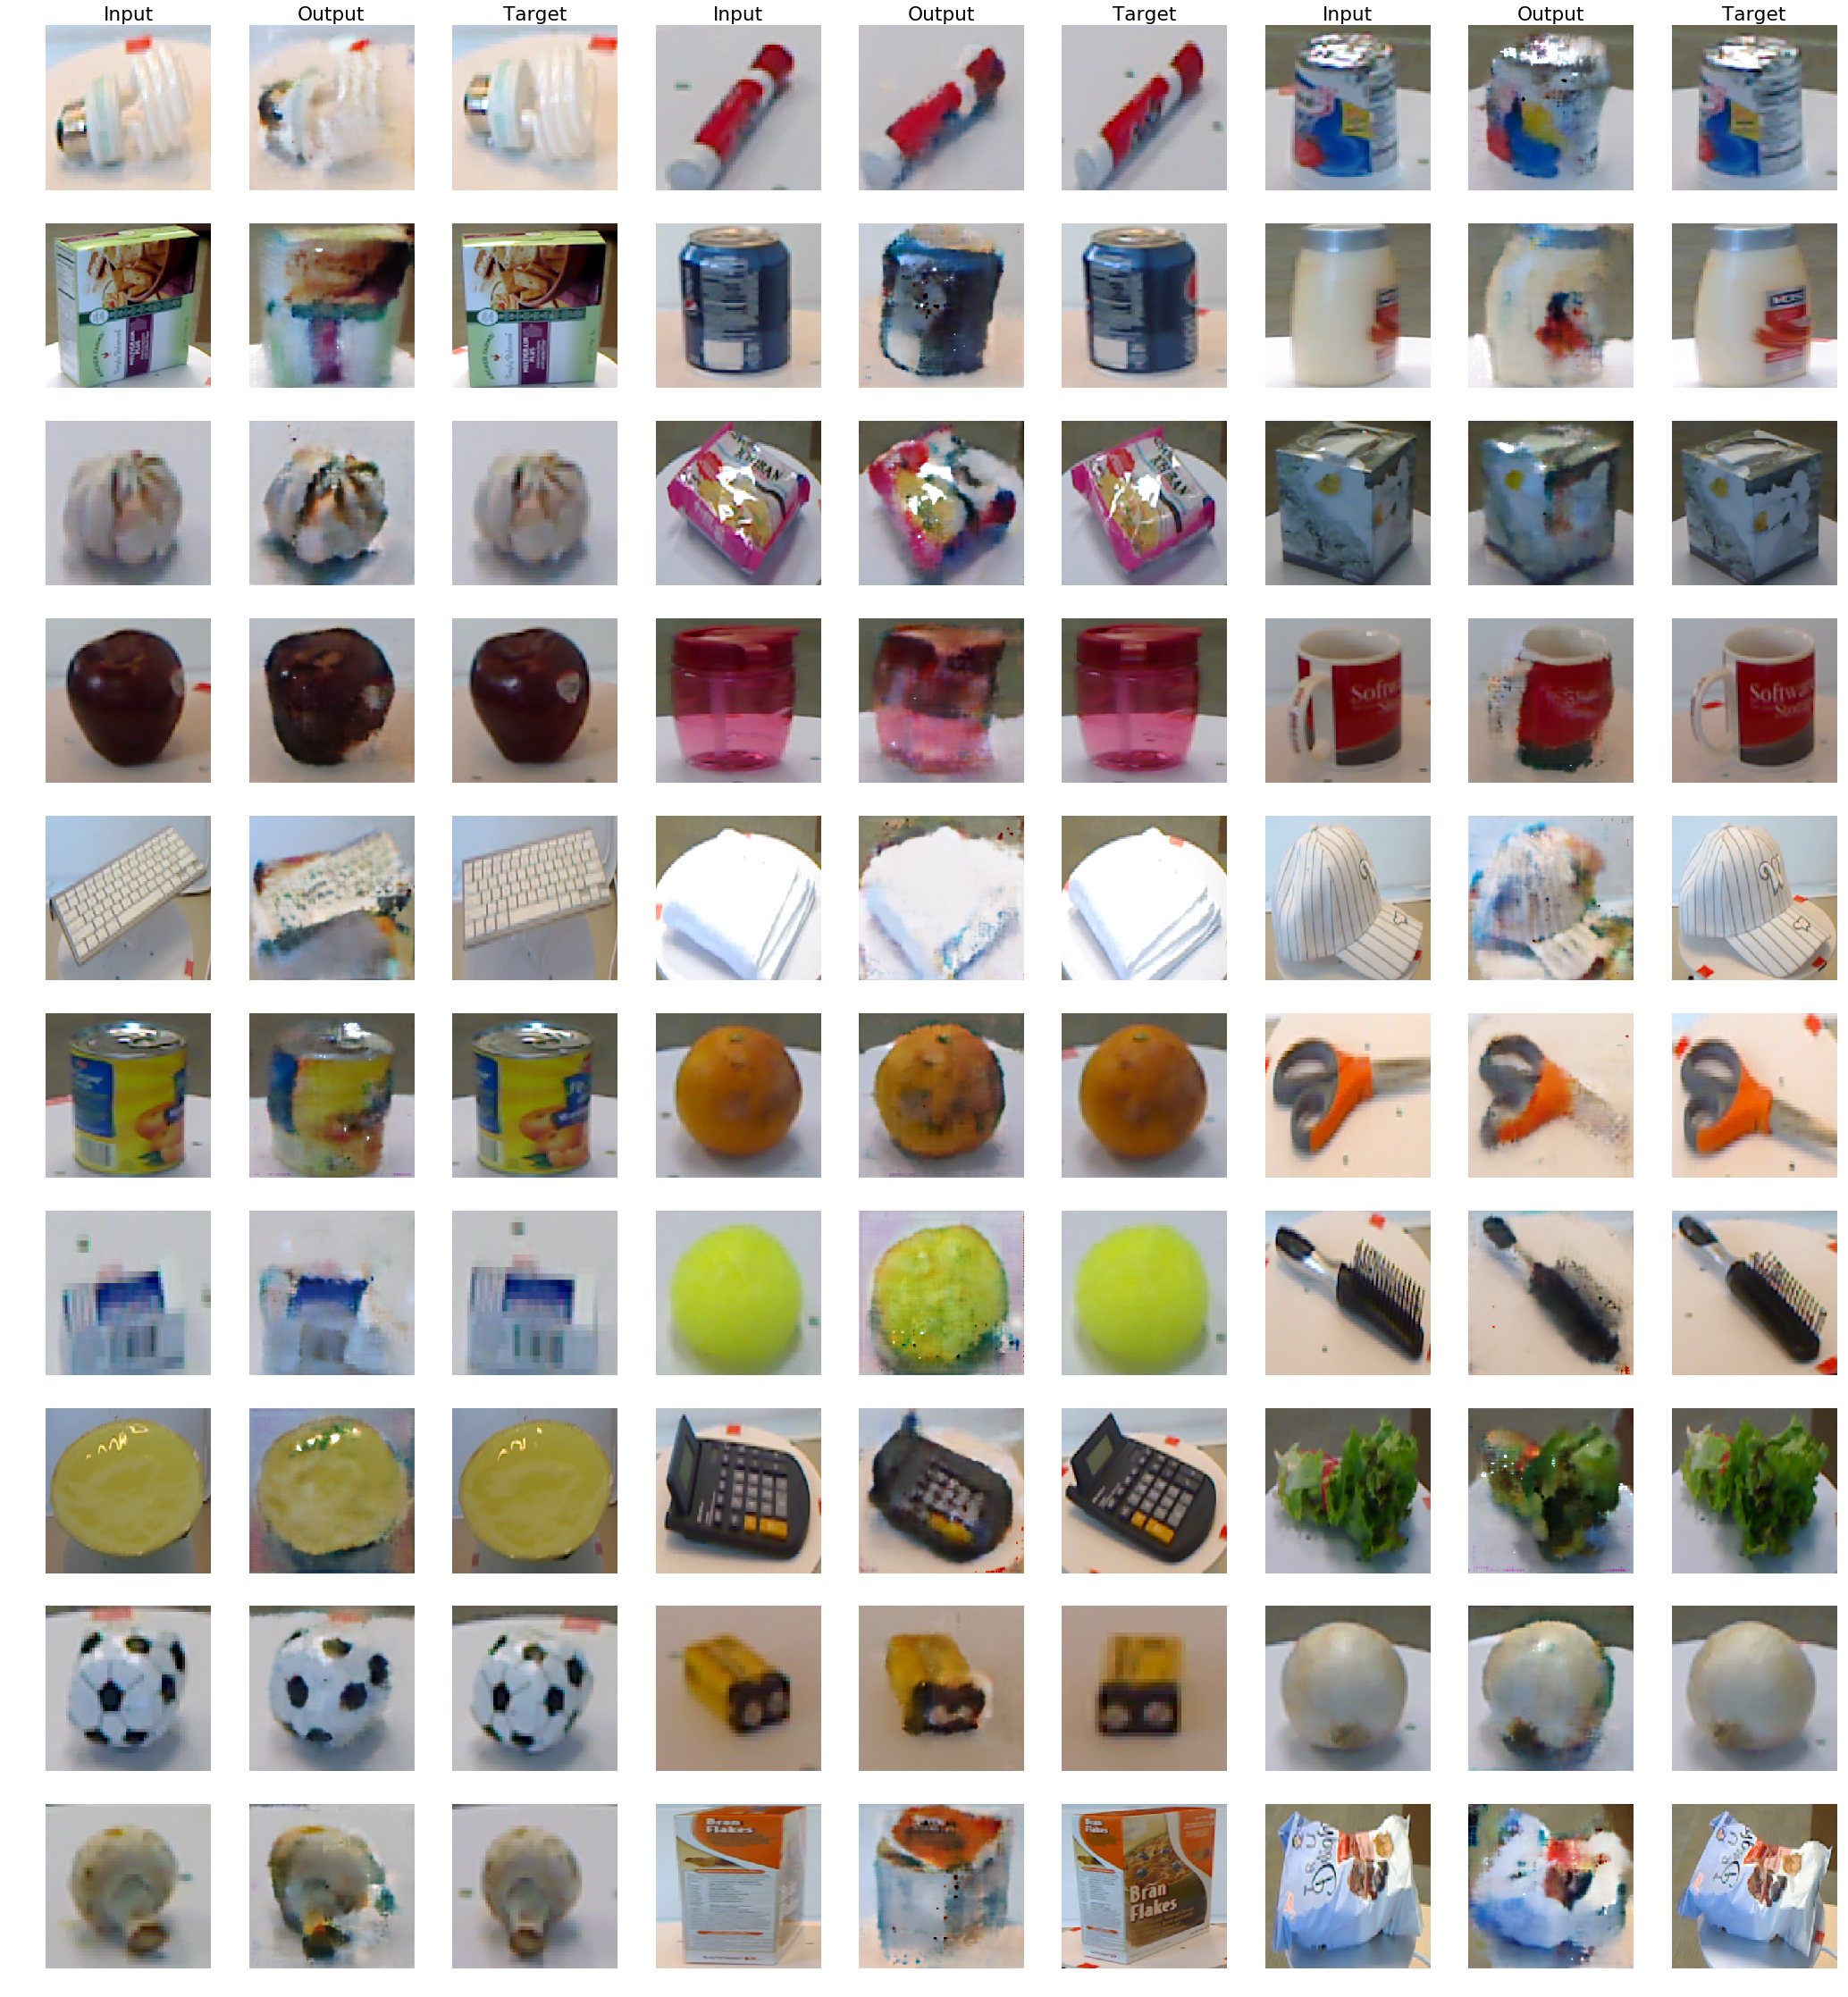
\includegraphics[width=\linewidth]{gan_pose_samples}
	\caption{Some generated samples from Pose-GAN trained with 50\% data. Note: The actual
		input is a 4-D image with the 4th dimension being the Depth-map, here we show only the
	RGB frame.}
	\label{fig:gan_pose_samples}
\end{figure}

\section{Performance of Depth-GAN Data}

In the first experiment, we try to reproduce Eitel et al. \cite{eitel}. We can
see the plotted results in Figure \ref{fig:eitel_accuracies}.

In general, we can see that \acrshort{gan} has good contribution in the classification
performance. It is worth mentioning that the transfer learning technique works very well,
so we still have the accuracies more than 80\% even when we use only 10\% of the data. It
is also expected to see the accuracies drop when we use only RGB data for training the
network, but the difference is only a few percentages, which is an indication that the
contribution of depth information is low in this training procedure. It is not a surprise
because the RGB channels themselves have already achieved a very high accuracy
(approximately 90\%). However, as other works also have shown \cite{eitel, alexandre},
depth information does help improving classification on \acrfull{cnn} when combining with
RGB, our experiment also follows that trend where all the accuracies using depth data are
higher in average than the corresponding results without depth.

\begin{table}[h!]
	\centering
	\caption{Dependent T-Test (rounded) results between different training experiments.
		For each block, Depth-GAN data is added to the training set (the
		right-hand-side numbers) and there is one experiment with only RGB data. All
		accuracies are compared with the result batch trained by the corresponding amount
		of original data. All values lower than 0.05 are highlighted.}
	\label{tab:t_test}
	\begin{tabular}{|l|l|l|}
		\hline
		Experiments      & p-values                        & Compared To            \\ \hline
		50 with only RGB & \textbf{0.0001} & \multirow{5}{*}{50-0}  \\ \cline{1-2}
		50-50            & \textbf{0.0156}   &                        \\ \cline{1-2}
		50-40            & \textbf{0.0220}   &                        \\ \cline{1-2}
		50-30            & 0.2173 			 &                        \\ \cline{1-2}
		50-20            & 0.9369 			 &                        \\ \hline
		25 with only RGB & \textbf{4.7233e-05} & \multirow{2}{*}{25-0}  \\ \cline{1-2}
		25-75            & \textbf{2.4228e-05} &                        \\ \hline
		10 with only RGB & \textbf{1.2940e-05}  & \multirow{2}{*}{10-0}  \\ \cline{1-2}
		10-90            & \textbf{2.7698e-06} &                        \\ \hline
		50-50            & 0.1249				& \multirow{3}{*}{100-0} \\ \cline{1-2}
		25-75            & 0.1803				&                        \\ \cline{1-2}
		10-90            & \textbf{0.0006}  	&                        \\ \hline
	\end{tabular}
\end{table}

It can be seen from Figure~\ref{fig:eitel_accuracies} that the absolute mean accuracies of
the classification noticeably increases when we add the \acrshort{gan} synthesized data to
the training set. In order to verify that, we run a Dependent T-test for the relevant
experiments to see if the accuracies significantly change or not. The reason why we choose
the Dependent Test is that our statistics are the results of the same experiment
(Evaluating a Deep Neural Network) under different settings. So using the Test for Paired
Samples is reasonable.

\begin{figure}[h!]
	\caption{Classification accuracies on Washington Dataset in different settings,
		trained and tested in 10 stratified random splits. The left number in a pair indicates
		the proportion of real data, and the right number indicates the proportion of synthesized
	data added.}
	\centering
	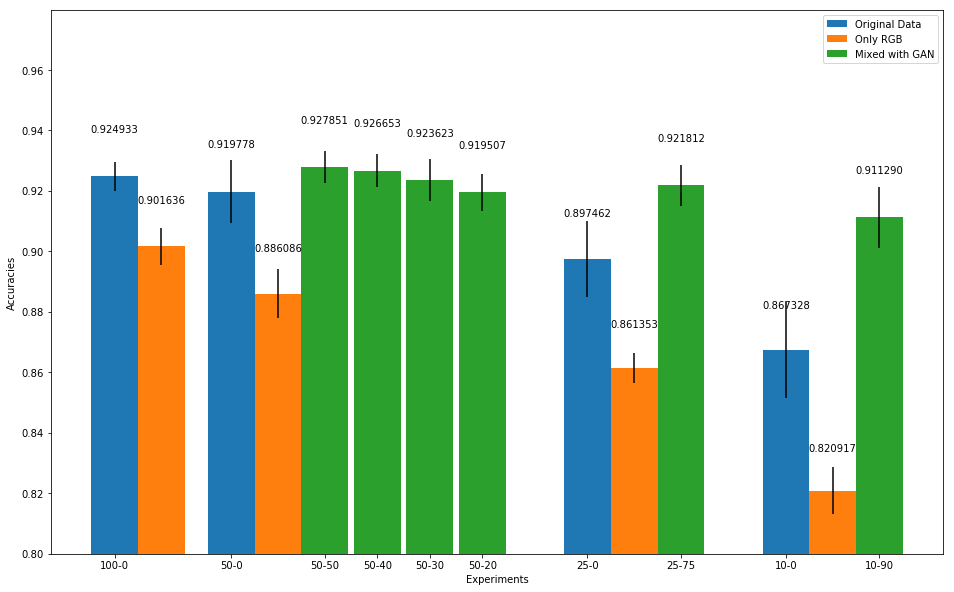
\includegraphics[width=0.9\textwidth]{img/eitel_accuracies}
	\label{fig:eitel_accuracies}
\end{figure}

\begin{figure}[h!]
	\centering
	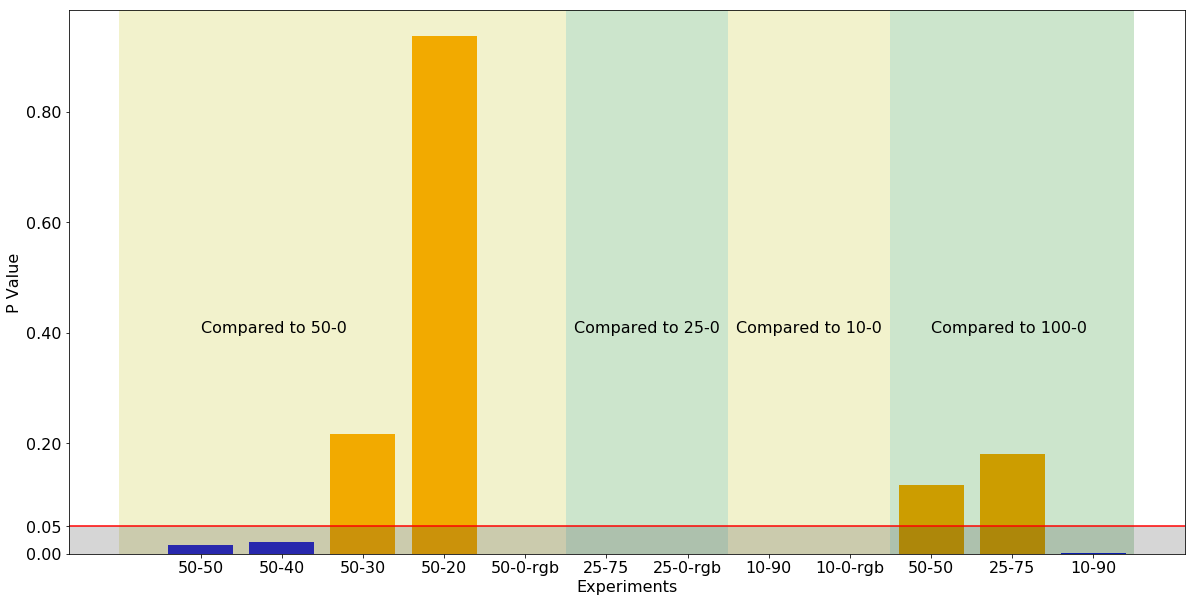
\includegraphics[width=0.9\linewidth]{t_test_plot}
	\caption{Visualization of table \ref{tab:t_test}. The blue bars are lower
	and the orange bars are higher than 0.05. 
	%Most of the important proportions of \acrshort{gan} data produce significantly
	%different accuracies (higher).  When comparing with the whole original data, only the
	%10-90 case yields a significantly different accuracy (lower). 
	Note: Some values are too small that they do not show clearly in this plot (see table
	\ref{tab:t_test}), but the important point is they are much smaller than 0.05 (the red
line)}
\label{fig:t_test_plot}
\end{figure}

In Figure~\ref{fig:eitel_accuracies}, there are 14 different experiments. We definitely do
not test every pair of experiments there, but instead only compare the results involving
\acrshort{gan} (the green bars) with the results with original data (the blue bars). In
this way, we would like to verify if training with \acrshort{gan} data is significantly
better than training without it. A significant level of 0.05 is used in all the tests. The
null hypothesis is "the 2 set of results are equal". In this statistical test, we combine
both the T-test and the mean accuracies plot in \ref{fig:eitel_accuracies} to reach a  
conclusion. If the test says that we can reject the null hypothesis, we conclude that the
one having higher mean is significantly better than the one having lower mean.

We can see in Table \ref{tab:t_test}, or even more clearly in the visualized version in
Figure \ref{fig:t_test_plot}, the T-test p-values for the experiments plotted in
Figure~\ref{fig:eitel_accuracies}. Based on those plots, we can conclude which strategies
significantly improve the classification training procedure.

In the case of 50\% of the original data, following the significant level of 0.05, we can
reject the null hypothesis for the case of 50-50, 50-40, and 50 with only RGB, meaning
they are significantly different from the results of 50-0.  As the plot in
Figure~\ref{fig:eitel_accuracies} shows higher mean values for 50-50 and 50-40 and lower
value for 50 with only RGB, it is reasonable to conclude that adding those proportions of
\acrshort{gan} data improves training the classifier significantly, and adding depth data
to the training indeed adds important values to the network. In this case we add
incremental amounts of \acrshort{gan} data (20\%, 30\% and 40\%) to see the trend of
\acrshort{gan}'s contribution. The accuracy plot \ref{fig:eitel_accuracies}, together with
the T-test results \ref{tab:t_test}, shows a clear incremental contribution with respect
to the amount of \acrshort{gan} data.

For the cases of 25\% and 10\% of original data, we only experiment with the full amount of
\acrshort{gan} data. The p-values are even more significantly lower than 0.05, indicating
that the results we have by adding 75\% and 10\%, respectively, of the training data from
our \acrshort{gan} are strongly better than the accuracies without them. The p-values of
the training with only RGB still shows the same trend with the 50\% case, saying that it
is meaningful to use Depth data in training our Object Classifier.

In addition, we also compare the results from full-combination results (i.e. 50-50, 25-75
and 10-90) with the accuracies of the classifier trained from 100\% of the original data
from the Washington RGB-D dataset. The p-values are in the last 3 rows of Table
\ref{tab:t_test}. We can only reject the null hypothesis in the case of 10-90.
Statistically, we cannot conclude that our accuracies with 50-50 and 25-75 are equal to
that of 100-0, but we have a strong base for saying that our \acrshort{gan} data can train
a comparable classifier with the optimal case. Only the 10-90 data shows a significantly
lower accuracies than 100-0, which is understandable as this Depth-GAN is trained with
only 10\% of the data which is probably not enough for it to capture the whole data
space. It is also one of the limitations of our experiment strategies, which is already
discussed in section \ref{sec:train_test_split}.


\section{Contribution of Depth Data in the Baseline Classifier}
In the previous section, we have already seen that the depth data from \acrshort{gan} helps
improving the classification performance in an RGB-Depth two-channel Deep Neural Network.
However, it was still not clear how much Depth Data contributes to the task. This is
important because if the network only learns from RGB data, our previous results do not
make too much sense and do not prove that our Depth-GAN is learning good Depth
Representations. A good news is, the previous experiments also revealed that the accuracies
achieved using only the RGB channels are significantly lower than with Depth involved. 

In this section, we would like to clarify how Depth contributes to the learning process by
doing a noise injection to the evaluation procedure of the Object Classification network.
We add Gaussian noises with mean 0 and standard deviations of 5, 10, 15, 20, and 40 respectively 
to the RGB, Depth, and both RGB and Depth channels of the Test Set and observe the
behaviors of the Deep Network during the Evaluation process. 

\begin{figure}[h!]
	\centering
	\begin{subfigure}{0.32\textwidth}
		\centering
		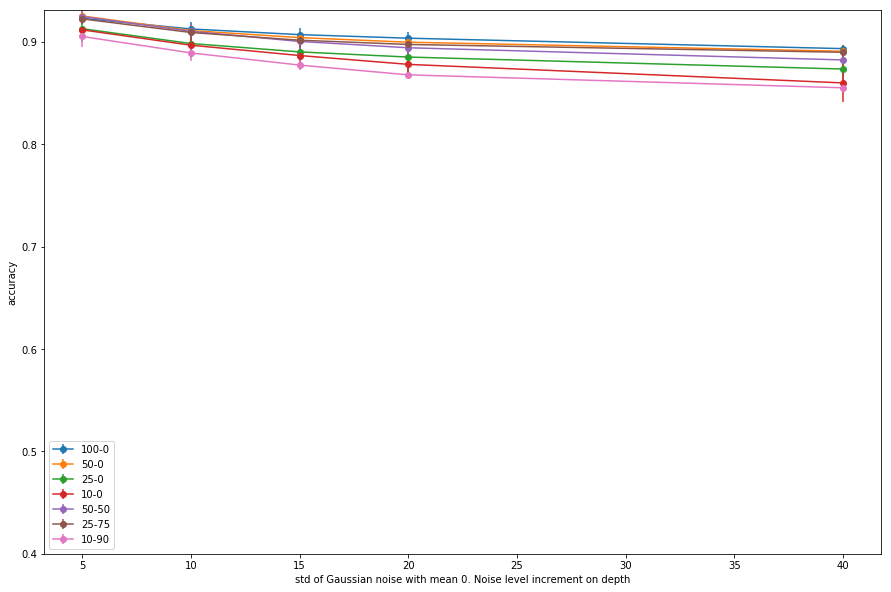
\includegraphics[width=\textwidth]{img/noise_injection_depth}
		\caption{Adding noises to depth}
	\end{subfigure}
	\begin{subfigure}{0.32\textwidth}
		\centering
		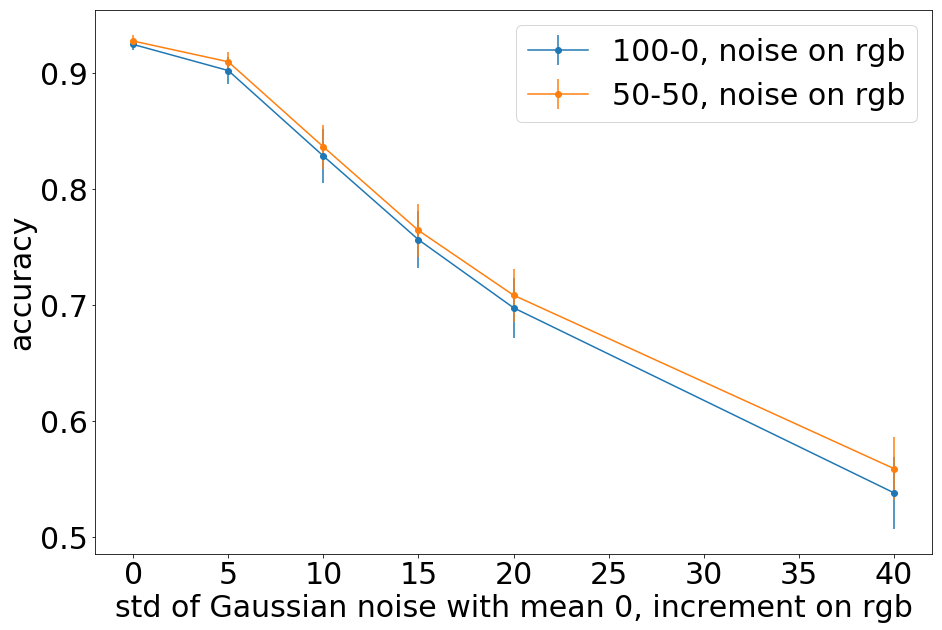
\includegraphics[width=\textwidth]{img/noise_injection_rgb}
		\caption{Adding noises to RGB}
	\end{subfigure}
	\begin{subfigure}{0.32\textwidth}
		\centering
		\includegraphics[width=\textwidth]{img/noise_injection_both}
		\caption{Adding noises to both channels}
		\label{subfig:noise_both}
	\end{subfigure}
	\caption{Noise Injection experiments. When adding noise to Depth, we experiment with
	the original training set (100-0) and all the combinations involving synthesized
depth. In the other two noise experiments, we perform them on only the original training
set and the strongest combination of synthesized depth (50-50) as we expect similar
behaviors from the combinations of synthesized depth. Note: The scales of 3 figures are
different.}
	\label{fig:noise_injection}
\end{figure}

Figure~\ref{fig:noise_injection} summarizes the behaviors of different experiments. There
are clearly different trends between adding noises to Depth and adding noises to RGB. When
adding noises to the RGB channels, the decrement of accuracies is more linear, whereas
when adding noises to the Depth channel, it is only linear up to a standard deviation of
20. Between 20 and 40, the decrement clearly vanishes, indicating that we are reaching a
limit of Depth contribution. In the same scale of noises, the behavior of the network when
we add noises to the RGB channels is different, it is almost a straight line from 5 to 40.
Figure~\ref{subfig:noise_both} shows a very similar pattern (to RGB) when we add noises to
both channels, which means RGB are the dominant channels here. In addition,
Figure~\ref{fig:noise_injection_2_channels} compares the rate of decrement when putting
the noise injection behaviors of the same dataset (50-50) in the same scale. The injection
to RGB is much steeper than the injection to Depth.

\begin{figure}[h!]
	\centering
	\includegraphics[width=0.9\linewidth]{noise_injection_2_separate_channels}
	\caption{Noise Injection on RGB and Depth separately, performing on the same
	synthesized depth combination and visualized in the same scale.}
	\label{fig:noise_injection_2_channels}
\end{figure}

\section{Performance of Pose-GAN Data \label{sec:performance_pose}}

For Pose-GAN, we train the baseline classifier with only the 50-50 proportion. Although
the resulting images look reasonable, they are still not perfect. There are many blurry
details, especially in complex objects such as the cereal box with textures and the comb,
or in objects with very similar color with the background such as the towel and the rubber
eraser. Therefore, it is not a surprise that we achieve only an accuracy of 66\% when
training the object classifier with the \acrshort{gan} data. As this is a very bad overall
accuracy and because of time limitation, we do not go further to perform the same
experiments as what we do with Depth-GAN. However, it is probably a good idea to look at
the category-wise accuracies to see which categories are easy for the \acrshort{gan} to learn
and which are not.

\begin{figure}[h!]
	\centering
	\includegraphics[width=\linewidth]{pose_gan_accuracies}
	\caption{Category-wise accuracies of the original data (Left) and Pose-GAN Data in
		50-50 proportion (Right). All the categories that the Pose-GAN performance is
		acceptable are highlighted in blue. By "acceptable" we mean that the accuracies is within
	a 0.1 error bound compared with the original data.}
	\label{fig:pose_gan_accuracies}
\end{figure}

In Figure~\ref{fig:pose_gan_accuracies}, only a few categories are
as-well-or-better classified using the data from the Pose-GAN, which means this
\acrshort{gan} is still not good enough to capture the entire 3D space representation,
although most of the synthesized RGB images are still distinguishable by human eyes (see
Figure \ref{fig:gan_pose_samples}).

We demonstrate some categories that the Pose-GAN performs quite well in
Figure~\ref{fig:acceptable}. Most of the synthesized objects still have problems with
complex details, but some of them are very fine. The calculator, for instance, is
well-rotated and can be clearly detected by human eyes; and the details such as the keypad
are still adequate. The Bell Pepper is almost perfect, but it is a round object so it is
easier for the Generator to learn. The Coffee Mug is successfully rotated, but loses all
the sharp textures.

\begin{figure}[h!]
	\centering
	\begin{subfigure}{0.32\textwidth}
		\includegraphics[width=\textwidth]{acceptable/bell_pepper_1_1_12}
		\caption{Bell Pepper}
	\end{subfigure}
	\begin{subfigure}{0.32\textwidth}
		\includegraphics[width=\textwidth]{acceptable/calculator_2_1_2}
		\caption{Calculator}
	\end{subfigure} 
	\begin{subfigure}{0.32\textwidth}
		\includegraphics[width=\textwidth]{acceptable/cap_1_1_2}
		\caption{Cap}
	\end{subfigure} 
	\begin{subfigure}{0.32\textwidth}
		\includegraphics[width=\textwidth]{acceptable/cereal_box_1_1_2}
		\caption{Cereal Box}
	\end{subfigure} 
	\begin{subfigure}{0.32\textwidth}
		\includegraphics[width=\textwidth]{acceptable/coffee_mug_1_1_5}
		\caption{Coffee Mug}
	\end{subfigure} 
	\begin{subfigure}{0.32\textwidth}
		\includegraphics[width=\textwidth]{acceptable/food_box_1_1_14}
		\caption{Food Box}
	\end{subfigure} 
	\begin{subfigure}{0.32\textwidth}
		\includegraphics[width=\textwidth]{acceptable/food_jar_1_1_14}
		\caption{Food Jar}
	\end{subfigure} 
	\begin{subfigure}{0.32\textwidth}
		\includegraphics[width=\textwidth]{acceptable/greens_1_1_5}
		\caption{Greens}
	\end{subfigure} 
	\begin{subfigure}{0.32\textwidth}
		\includegraphics[width=\textwidth]{acceptable/pear_1_1_3}
		\caption{Pear}
	\end{subfigure} 
	\begin{subfigure}{0.32\textwidth}
		\includegraphics[width=\textwidth]{acceptable/pitcher_2_1_2}
		\caption{Pitcher}
	\end{subfigure} 
	\begin{subfigure}{0.32\textwidth}
		\includegraphics[width=\textwidth]{acceptable/scissors_1_1_2}
		\caption{Scissors}
	\end{subfigure} 
	
	\caption{Samples from the categories in which the synthesized objects produce
		acceptable accuracies, in figure \ref{fig:pose_gan_accuracies}. On the left are
	the original objects, on the right are the rotated pose produced by Pose-GAN.}
	\label{fig:acceptable}
\end{figure}

\begin{figure}[h!]
	\centering
	\begin{subfigure}{0.32\textwidth}
		\includegraphics[width=0.8\linewidth]{not_acceptable/food_can_1_1_14}
		\caption{Food Can}
	\end{subfigure}
	\begin{subfigure}{0.32\textwidth}
		\includegraphics[width=0.8\linewidth]{not_acceptable/garlic_1_1_15}
		\caption{Garlic}
	\end{subfigure}
	\begin{subfigure}{0.32\textwidth}
		\includegraphics[width=0.8\linewidth]{not_acceptable/glue_stick_1_1_2}
		\caption{Glue Stick}
	\end{subfigure}
	\begin{subfigure}{0.32\textwidth}
		\includegraphics[width=0.8\linewidth]{not_acceptable/instant_noodles_2_1_14}
		\caption{Instant Noodles}
	\end{subfigure}
	\begin{subfigure}{0.32\textwidth}
		\includegraphics[width=0.8\linewidth]{not_acceptable/lemon_1_1_2}
		\caption{Lemon}
	\end{subfigure}
	\begin{subfigure}{0.32\textwidth}
		\includegraphics[width=0.8\linewidth]{not_acceptable/lightbulb_1_1_2}
		\caption{Light Bulb}
	\end{subfigure}
	\begin{subfigure}{0.32\textwidth}
		\includegraphics[width=0.8\linewidth]{not_acceptable/lime_1_1_8}
		\caption{Lime}
	\end{subfigure}
	\begin{subfigure}{0.32\textwidth}
		\includegraphics[width=0.8\linewidth]{not_acceptable/orange_1_1_2}
		\caption{Orange}
	\end{subfigure}
	\begin{subfigure}{0.32\textwidth}
		\includegraphics[width=0.8\linewidth]{not_acceptable/rubber_eraser_1_1_2}
		\caption{Rubber Eraser}
	\end{subfigure}
	\begin{subfigure}{0.32\textwidth}
		\includegraphics[width=0.8\linewidth]{not_acceptable/shampoo_1_2_4}
		\caption{Shampoo}
	\end{subfigure}
	\begin{subfigure}{0.32\textwidth}
		\includegraphics[width=0.8\linewidth]{not_acceptable/pliers_2_1_3}
		\caption{Pliers}
	\end{subfigure}
	\begin{subfigure}{0.32\textwidth}
		\includegraphics[width=0.8\linewidth]{not_acceptable/stapler_2_1_2}
		\caption{Stapler}
	\end{subfigure}
	
	\caption{Samples from the categories in which the synthesized objects does not produce
		good results in figure \ref{fig:pose_gan_accuracies}.}
	\label{fig:not_acceptable}
\end{figure}

On the contrary, Figure~\ref{fig:not_acceptable} shows some examples of the objects
behaving much worse in the classifier than the original data.  Among the failed ones, only
The Light Bulb and the Glue Stick are indeed bad. They do not have a clear shape and are
not clearly distinguishable from the background. The rest of them still look quite nice,
such as the Instant Noodles, the Stapler and the Rubber Eraser. The Shampoo and the Food
Can are not as good as the two above, but are still better, or at least comparable to the
Cap and the Food Box in Figure~\ref{fig:acceptable}. An observed phenomenon is that
regardless of how we train the Pose-GAN, the classification results of those categories
are still equally bad, although the visual outcomes do improve noticeably as we apply more
regularization tricks. This raises an interesting question on why the classifier fails to
correctly recognize the synthesized images while they still look very good to human eyes;
and at the same time performs greatly with the real counterparts. More work might need to
be done in order to find the reason why they behave differently while sharing similar
appearance qualities. 

Because we remove 17 categories from the Pose-GAN's training set as being mentioned in
section \ref{sub:training_gan}, we also try to make it a fairer game by also removing the
same categories from the training and test sets of the classifier. However, the results of
the remaining categories show no differences from what we have discussed above.

    %! TEX root = /home/duy/TUB/Thesis/latex-source/DiplomarbeitLaTex.tex

\chapter{Conclusion and Future Work \label{cha:conclusion}}

Our experiments show that Depth Data is contributive and adding depth data
from our Depth-GAN is beneficial to training an Object Classifier to different extents. 
It is worth noting that, because of a drawback of our train-test split explained in
section \ref{sec:train_test_split}, our \acrshort{gan}s creating different proportions
are not equal. This is clearly demonstrated in section \ref{sub:depth_gan}. However,
despite the disadvantages it has, the \acrshort{gan} trained by 10\% of the data still
performs greatly by improving the classification results significantly, comparing to the
classifier trained on only 10\% of the original data. The same is true for the
\acrshort{gan} trained with 25\% of the original data.

Therefore, the Depth-GAN is particularly useful when our "real" training data is not
complete and the synthesized data is added in a large proportion, such as the 10-90 case.
It is a good idea to synthesize the depth-maps when we have a large training set but only
a small portion of images have depth-maps included or there is even no depth-maps at all.

In the way around, if we consider the baseline classifier as a quantitative tool to
evaluate \acrshort{gan} data, then our Depth-GAN is showing its potentials. The results
are good in both ways: to human eyes, as demonstrated in Figure~\ref{fig:gan_depth}, and
in quantitative metrics, shown in the accuracies plot \ref{fig:eitel_accuracies} and
T-Test results \ref{tab:t_test}.

The Pose-GAN, in another way, only does a good job on some particular objects. It is
understandable as its task is much more complicated than the Depth-GAN and other
\acrshort{pix} applications. It is not a simple Image-to-Image translation task, but
requires a good representation of the 3D space. Although we have provided the depth map
(as the 4th dimension), the Pose-GAN still does not utilize this information well and
cannot capture the full 3D space distribution of the objects. A reason could be that this
setting (4-dimensional image with 4 channels R,G,B, and D) is still not optimal. A
reasonable future work is to try another depth representation when training the Pose-GAN.

Beside some very poorly produced objects, there are some categories which the Pose-GAN
still does a decent job, as we have discussed in section \ref{sec:performance_pose}. There
is still questions left on why there is such a big difference on classification
performance between synthesized and real images although they look quite similar. One
possible approach is to inspect the color distribution of the synthesized images and
verify if there is any major deviation from that of the real images. A further and more
costly step could be tracing the layers of the classifier and/or the Discriminator to spot
the points where things go wrong. Because \acrshort{gan}s do not minimize a single scalar
loss function which the classifier uses, there could be some level of mismatching between
the two.

While training the baseline classifier with both the original and the synthesized data, we
observe a behavior that the network learns much more from the RGB channels than the Depth
one. We tried to regularize the RGB channels in different ways, such as adding Gaussian
Noise to the RGB frame and Dropouts, but could not change the Network's learning behavior.
Similar to the point above, using another representation of Depth instead of colorizing
and treating it as a second RGB frame, could be the answer and could improve the
classification results even further.

Furthermore, as the Discriminator of \acrshort{gan}s is trained to perform good
classification between real data and the synthesized data from the Generator, it can also
contain layers with useful information about the dataset. Another feasible future work is
to take the weight vectors of one or a few layers before the Softmax as the
representations for other tasks, such as our baseline classification.



% ---------------------------------------------------------------
\backmatter % no page numbering from here
    %\addchap{List of Acronyms}

\begin{tabbing}
spacespacespace \= space \kill
GAN \> Generative Adversarial Networks \\
ML \> Machine Learning \\
VAE\> Variational Auto Encoder \\
DL \> Deep Learning \\
Pix2Pix \> Image-to-Image Translation with Conditional Adversarial Networks \\
AI \> Artificial Intelligence \\
MSE \> Mean Squared Error \\
CNN \> Convolutional Neural Networks \\
HOG  \> Histogram of Gradients \\
\end{tabbing}
\endinput

		
		% if you want to provide a glossary with explanations of important terms put it in here

    %\bibliographystyle{geralpha}
    \bibliographystyle{plain}
    \bibliography{./bib/references}
    
    %\addchap{Annex}

\begin{appendix}

\lstset{language=,caption=Sourcecode Listing,captionpos=b,
label=yahoowidgetkon,showstringspaces=false,
basicstyle={\fontfamily{pcr}\selectfont\footnotesize}}
\begin{lstlisting}
<?xml version="1.0" encoding="UTF-8"?>
<widget>
	 <debug>off</debug>
	 <window name="myWindow" title="Hello Widget" visible="true">
		 <height>120</height>
		 <width>320</width>
		 <image src="Resources/orangebg.png">
			<name>orangebg</name>
			<hOffset>0</hOffset>
			<vOffset>0</vOffset>
		</image>
		 <text>
			 <name>myText</name>
			 <data>Hello Widget</data>
			 <color>#000000</color>
			 <size>20</size>
			 <vOffset>50</vOffset>
			 <hOffset>120</hOffset>
		 </text>
	</window>
</widget>
\end{lstlisting}

\newpage


\lstset{caption=SIP request and response packet\cite{SIPBook},
captionpos=b,label=sippacket,showstringspaces=false,
basicstyle={\fontfamily{pcr}\selectfont\footnotesize}}
\begin{lstlisting}
INVITE sip:bob@network.org SIP/2.0
Via: SIP/2.0/UDP 100.101.102.103:5060;branch=z9hG4bKmp17a
Max-Forwards: 70
To: Bob <sip:bob@network.org>
From: Alice <sip:alice@ims-network.org>;tag=42
Call-ID: 10@100.101.102.103
CSeq: 1 INVITE
Subject: How are you?
Contact: <sip:xyz@network.org>
Content-Type: application/sdp
Content-Length: 159
v=0
o=alice 2890844526 2890844526 IN IP4 100.101.102.103
s=Phone Call
t=0 0
c=IN IP4 100.101.102.103
m=audio 49170 RTP/AVP 0
a=rtpmap:0 PCMU/8000

SIP/2.0 200 OK
Via: SIP/2.0/UDP proxy.network.org:5060;branch=z9hG4bK83842.1
;received=100.101.102.105
Via: SIP/2.0/UDP 100.101.102.103:5060;branch=z9hG4bKmp17a
To: Bob <sip:bob@network.org>;tag=314159
From: Alice <sip:alice@network.org>;tag=42
Call-ID: 10@100.101.102.103
CSeq: 1 INVITE
Contact: <sip:foo@network.org>
Content-Type: application/sdp
Content-Length: 159
v=0
o=bob 2890844526 2890844526 IN IP4 200.201.202.203
s=Phone Call
c=IN IP4 200.201.202.203
t=0 0
m=audio 49172 RTP/AVP 0
a=rtpmap:0 PCMU/8000
\end{lstlisting}


\end{appendix}

\endinput


\end{document}
